% Options for packages loaded elsewhere
\PassOptionsToPackage{unicode}{hyperref}
\PassOptionsToPackage{hyphens}{url}
\PassOptionsToPackage{dvipsnames,svgnames,x11names}{xcolor}
\documentclass[
  letterpaper,
  11pt]{article}
\usepackage{xcolor}
\usepackage[margin=1in]{geometry}
\usepackage{amsmath,amssymb}
\setcounter{secnumdepth}{-\maxdimen} % remove section numbering
\usepackage{iftex}
\ifPDFTeX
  \usepackage[T1]{fontenc}
  \usepackage[utf8]{inputenc}
  \usepackage{textcomp} % provide euro and other symbols
\else % if luatex or xetex
  \usepackage{unicode-math} % this also loads fontspec
  \defaultfontfeatures{Scale=MatchLowercase}
  \defaultfontfeatures[\rmfamily]{Ligatures=TeX,Scale=1}
\fi
\usepackage{lmodern}
\ifPDFTeX\else
  % xetex/luatex font selection
\fi
% Use upquote if available, for straight quotes in verbatim environments
\IfFileExists{upquote.sty}{\usepackage{upquote}}{}
\IfFileExists{microtype.sty}{% use microtype if available
  \usepackage[]{microtype}
  \UseMicrotypeSet[protrusion]{basicmath} % disable protrusion for tt fonts
}{}
\makeatletter
\@ifundefined{KOMAClassName}{% if non-KOMA class
  \IfFileExists{parskip.sty}{%
    \usepackage{parskip}
  }{% else
    \setlength{\parindent}{0pt}
    \setlength{\parskip}{6pt plus 2pt minus 1pt}}
}{% if KOMA class
  \KOMAoptions{parskip=half}}
\makeatother
\usepackage{longtable,booktabs,array}
\newcounter{none} % for unnumbered tables
\usepackage{calc} % for calculating minipage widths
% Correct order of tables after \paragraph or \subparagraph
\usepackage{etoolbox}
\makeatletter
\patchcmd\longtable{\par}{\if@noskipsec\mbox{}\fi\par}{}{}
\makeatother
% Allow footnotes in longtable head/foot
\IfFileExists{footnotehyper.sty}{\usepackage{footnotehyper}}{\usepackage{footnote}}
\makesavenoteenv{longtable}
\usepackage{graphicx}
\makeatletter
\newsavebox\pandoc@box
\newcommand*\pandocbounded[1]{% scales image to fit in text height/width
  \sbox\pandoc@box{#1}%
  \Gscale@div\@tempa{\textheight}{\dimexpr\ht\pandoc@box+\dp\pandoc@box\relax}%
  \Gscale@div\@tempb{\linewidth}{\wd\pandoc@box}%
  \ifdim\@tempb\p@<\@tempa\p@\let\@tempa\@tempb\fi% select the smaller of both
  \ifdim\@tempa\p@<\p@\scalebox{\@tempa}{\usebox\pandoc@box}%
  \else\usebox{\pandoc@box}%
  \fi%
}
% Set default figure placement to htbp
\def\fps@figure{htbp}
\makeatother
\setlength{\emergencystretch}{3em} % prevent overfull lines
\providecommand{\tightlist}{%
  \setlength{\itemsep}{0pt}\setlength{\parskip}{0pt}}
% =============================================================================
% Custom preamble for ConductorBlindSpot (pandoc -> XeLaTeX)
% Pulled in via `--include-in-header` by build.ps1 / build.sh.
%
% This file is injected into pandoc's default LaTeX template at the
% `header-includes` slot, which runs BEFORE pandoc's own \usepackage{hyperref}
% and \usepackage{unicode-math}. We therefore:
%   * load `mathtools` here (so it precedes unicode-math, per its manual),
%   * defer any \hypersetup{...} with \AtBeginDocument{...}.
% We only ADD or tune; we do not reload packages pandoc already loads
% (amsmath, amssymb, amsfonts, hyperref, xcolor, fontspec, unicode-math).
% =============================================================================

% ---- Math / symbols (mathtools must precede unicode-math) ------------------
\usepackage{mathtools}
\usepackage{amsthm}

% ---- Typography -------------------------------------------------------------
\usepackage{microtype}
\usepackage{booktabs}

% ---- TikZ for the few embedded figures (loaded for both papers; harmless if
% no tikzpicture environment appears in the source) -------------------------
\usepackage{tikz}
\usetikzlibrary{positioning,arrows.meta}
% Let LaTeX stretch lines a bit further when it can't find a clean break;
% keeps overfull hboxes out of display math and URL-heavy lines.
\setlength{\emergencystretch}{3em}
% Make long URLs breakable at hyphens (applied before hyperref loads), and load
% xurl so they also break at any character -- a single long no-hyphen URL (e.g.
% the bare GitHub link) would otherwise run 40+pt into the margin.
\PassOptionsToPackage{hyphens}{url}
\usepackage{xurl}

% ---- Hebrew letter support (for the simplicial-series labels ל0–ל7) --------
% Latin Modern Roman lacks Hebrew glyphs; without this, xelatex emits
% "missing character" warnings and leaves the slots blank. \heb{...} switches
% to a system font with Hebrew coverage (Times New Roman, ships with Windows)
% for the wrapped text only, and is declared *robust* so hyperref / titling do
% not try to expand it during protected-edef of moving arguments. The accsupp
% ActualText annotation makes the glyph ל extract as "L" for PDF-to-text and
% screen readers while the rendered glyph stays ל. (Mirrors the simplicial build.)
\usepackage{accsupp}
\providecommand{\hebrewfont}{}
\DeclareRobustCommand{\heb}[1]{%
  \BeginAccSupp{ActualText=L}{\hebrewfont #1}\EndAccSupp{}%
}
\AtBeginDocument{%
  \newfontfamily\HebrewSysFont{Times New Roman}[Scale=MatchLowercase]%
  \renewcommand{\hebrewfont}{\HebrewSysFont}%
}

% ---- Section heading polish -------------------------------------------------
\usepackage{titlesec}
\titleformat{\section}
  {\normalfont\Large\bfseries}{\thesection}{0.75em}{}
\titleformat{\subsection}
  {\normalfont\large\bfseries}{\thesubsection}{0.6em}{}
\titleformat{\subsubsection}
  {\normalfont\normalsize\bfseries}{\thesubsubsection}{0.5em}{}

% ---- Hyperref polish ----------------------------------------------------
% PDF metadata (pdftitle/pdfauthor/...) is driven by pandoc's -V flags
% (title/author from the front matter), so the preamble stays paper-neutral.

% ---- Theorem-like environments (available if source ever migrates) ---------
% The markdown source uses `**Theorem 4.1 (title).**` bold-header paragraphs
% rather than native environments, so these are currently unused by the body
% but are kept here so a future migration does not require a preamble change.
\theoremstyle{plain}
\newtheorem{theorem}{Theorem}[section]
\newtheorem{proposition}[theorem]{Proposition}
\newtheorem{lemma}[theorem]{Lemma}
\newtheorem{corollary}[theorem]{Corollary}
\newtheorem{conjecture}[theorem]{Conjecture}
\theoremstyle{definition}
\newtheorem{definition}[theorem]{Definition}
\theoremstyle{remark}
\newtheorem{remark}[theorem]{Remark}
\newtheorem{example}[theorem]{Example}

% --- Figure path resolution -------------------------------------------------
% Figures live under the repo root (empirical/apex_recovery/reports/...), but
% latexmk runs xelatex from build/. Search the parent (and a couple of fallbacks)
% so root-relative \includegraphics paths resolve regardless of invocation.
\usepackage{graphicx}
\graphicspath{{../}{./}{../../}}

% Encourage figures to share pages with text rather than floating to their own
% near-empty page (the default \floatpagefraction is too strict for medium figures).
\renewcommand{\topfraction}{0.9}
\renewcommand{\bottomfraction}{0.8}
\renewcommand{\textfraction}{0.07}
\renewcommand{\floatpagefraction}{0.7}
\setcounter{topnumber}{3}
\setcounter{totalnumber}{4}

% (The \heb{ל} macro, \emergencystretch, and url-hyphenation are already defined
% earlier in this shared preamble — used by both papers — so we do not redefine
% them here; BeyondTheConductorBlindSpot.md uses \heb{ל} for the lamed series.)

% Pull the title-page content up (smaller top margin) so the Keywords line that
% currently spills to page 2 fits on page 1. Applied after pandoc's geometry.
\geometry{top=0.8in}
\usepackage{bookmark}
\IfFileExists{xurl.sty}{\usepackage{xurl}}{} % add URL line breaks if available
\urlstyle{same}
\hypersetup{
  pdftitle={Beyond the Conductor Blind Spot: Eigenfunction Identifiability and Planning in Non-Gaussian Worlds},
  pdfauthor={Leonardo Murillo Montero},
  colorlinks=true,
  linkcolor={Maroon},
  filecolor={Maroon},
  citecolor={Blue},
  urlcolor={Blue},
  pdfcreator={LaTeX via pandoc}}

\title{Beyond the Conductor Blind Spot: Eigenfunction Identifiability and Planning in Non-Gaussian Worlds}
\author{Leonardo Murillo Montero}
\date{June 2, 2026}

\begin{document}
\maketitle
\begin{abstract}
The companion certificate \emph{The Conductor Blind Spot} proved a sharp, finite fact: on a categorical head whose outcomes carry a cyclic ring structure, the second-order curvature class --- the Fisher form shared by natural gradient, K-FAC, Adam's empirical Fisher, and gradient-based attribution --- is constitutionally unable to represent an order-three coupling (the Amari--Chentsov cubic) that the head's own information geometry carries. That statement is finite, exact, and lives on a discrete index. This paper asks, and answers, the continuous counterpart: \textbf{when a representation is learned by the generic self-supervised recipe --- pull positive pairs together, keep the embedding whitened --- what does it recover, and when is the second-order (linear) picture of that representation complete?}

We show that the \emph{population optimum} of this objective recovers, in each latent coordinate, the \emph{slowest eigenfunction} of the pair-generating transition operator, up to a rotation: a clean, model-free consequence of the Ky Fan maximum principle (a statement about the optimum, not about what a finite encoder trained by gradient descent reaches). That eigenfunction --- the \textbf{slow-feature chart}, the coordinate-free object the recovery is ``up to'' --- is a \textbf{straight line exactly when the latent law is Gaussian in the observed coordinate}, and a known, monotone, \emph{curved} coordinate otherwise. Three theorems follow. (i) \textbf{Exact recovery}: the optimum equals the slow-eigenfunction chart up to a block rotation, so a linear probe recovers the \emph{latent factors} if and only if the world is Gaussian in that coordinate, and is provably lossy otherwise (other downstream targets may still be linearly readable). (ii) \textbf{Approximate recovery}: under inexact whitening (\(\varepsilon\)) and inexact alignment (\(\delta\)), the chart is recovered within \((\varepsilon+\sqrt{2\delta/\gamma})^2\), where \(\gamma\) is the slow-feature spectral gap; the guarantee degrades gracefully and is governed by a checkable condition, not a tunable. (iii) \textbf{Planning}: because the recovered chart is a diffeomorphism, every optimal-control problem on the true latent transports \emph{exactly} into the learned coordinates --- planning in the representation equals planning in the world, with the warp applied when it is not the identity.

The unifying statement is that the conductor blind spot and the failure of linear probing share a \textbf{trigger of the same kind} --- departure from second-order sufficiency (\(\kappa_{\ge 3}\neq 0\)) --- and are \textbf{quantitatively linked} near the Gaussian; they are two registers of one boundary, offset by one in their order index and coinciding at the Gaussian corner. This is a correspondence of model classes that we \emph{measure} --- the finite order-three object regenerated exactly, the lock measured as a square law --- not a single diagnostic run end-to-end across both. We give deterministic, exact-arithmetic and numerical certificates for every claim; the finite-categorical certificate independently regenerates the conductor blind spot's published counts, and a cross-register certificate measures the two registers locking together --- the recovery-map curvature scales as the square of the leading distributional cumulant, vanishing with it at the Gaussian. A related signature is visible, unforced, in a pretrained language model, where it appears as a middle-layer phenomenon: the heavy non-Gaussian directions of the residual stream \emph{tend} to be those whose recovered slow feature is curved (a positive but imperfect rank correlation, not an identity --- and an observational check well outside the theorem's hypotheses). The consequences for practice --- interpretability (linear probes are provably partial off-Gaussian), optimization (the same order-two ceiling as the blind spot), and the auditing of learned world models (identifiability holds, but only up to a \emph{recoverable nonlinear} chart) --- are drawn out explicitly.

\textbf{Keywords:} self-supervised learning, identifiability, transition operator, slow feature analysis, eigenfunctions, Sturm--Liouville, information geometry, Amari--Chentsov cubic, Ky Fan, optimal control, world models.
\end{abstract}

{
\setcounter{tocdepth}{3}
\tableofcontents
}
\subsection{1. Introduction}\label{sec:intro}

\subsubsection{1.1 A finite fact, and its continuous shadow}\label{a-finite-fact-and-its-continuous-shadow}

The conductor blind spot is a statement one can check by hand on a clock. Index the outcomes of a categorical head by \(\mathbb{Z}/n\mathbb{Z}\) --- the hours of an \(n\)-hour clock, the months of a calendar, the residues of a modular-arithmetic task. At the uniform (maximum-entropy) point the Fisher information is diagonal in the additive-character basis, hence \emph{block-diagonal across conductor packets}; but the next form in the cumulant tower, the Amari--Chentsov cubic, couples those packets exactly when three frequencies sum to zero modulo \(n\). The cubic coupling is therefore real local structure that no second-order curvature surrogate can represent. That is the blind spot: an order-three fact invisible to an order-two instrument, certified in exact integer arithmetic.

It is natural to suspect that the same ceiling governs \emph{continuous} representation learning, where there is no ring and no exact integer certificate --- only a network trained to make the embeddings of two related views agree. This paper makes that suspicion precise. We do not transport the cyclic combinatorics; we ask the question the continuous setting actually poses and follow the mathematics to its own answer.

\subsubsection{1.2 The question, and the shape of the answer}\label{the-question-and-the-shape-of-the-answer}

A \emph{world} is a hidden variable \(z\) with a stationary law \(p\), observed through \emph{positive pairs} \((z,z')\) --- two augmentations of an image, two nearby frames of a video, two consecutive states of a process --- generated by a stationary, reversible, additive-noise transition. A learner sees only a scrambled observation \(x=g(z)\) and trains an encoder so that paired embeddings align while the embedding distribution stays whitened (the standard anti-collapse constraint). The question is what the trained encoder recovers of \(z\).

The answer has one moving part. Minimising alignment subject to whitening is, exactly, a Rayleigh quotient on the transition operator \(T\) that carries one view to the next; by the Ky Fan maximum principle its solution is the span of the \emph{slowest} non-constant eigenfunctions of \(T\). So the population optimum recovers the slow-eigenfunction chart of the world --- nothing more, nothing less. Whether that chart is the latent itself or a curved version of it is then decided by a single classical dichotomy:

\begin{quote}
the slowest eigenfunction of an additive-noise transition is an \textbf{affine} function of the latent \textbf{if and only if} the latent law is \textbf{Gaussian} (Sturm--Liouville);
for every other law it is a \textbf{monotone but curved} coordinate.
\end{quote}

The Gaussian is thus the one world where the recovered chart is the latent up to rotation --- where a \emph{linear} probe of the representation is complete. Everywhere else, recovery still succeeds, but through a recoverable nonlinear coordinate, and a linear probe necessarily discards content.

We fix here a convention that recurs throughout, because it is the one place a careful reader can trip. A representation is read by a \emph{linear probe} --- a degree-one map --- and that probe is complete exactly when the representation's \textbf{second-order statistics} (its covariance) determine the latent, which by Theorem 2 holds if and only if the world is Gaussian. So whenever we say ``second-order'' we mean \emph{the sufficiency of second-order statistics}, never the degree of the probe map (which is one) nor the order of the cumulant whose appearance defeats it (which is three). With that reading fixed, the linear-probe boundary is the continuous counterpart of the blind spot: a linear reading of the representation is complete exactly on the Gaussian (second-order-sufficient) stratum, and provably partial off it.

\subsubsection{1.3 Contributions}\label{contributions}

\begin{enumerate}
\def\labelenumi{\arabic{enumi}.}
\item
  \textbf{An exact recovery theorem} (§3, Appendix A.1--A.3). The whitened-alignment \emph{population optimum} equals the slow-eigenfunction chart \(\Phi_1\) up to a block rotation, under an explicit and checkable slow-feature gap. A gradient-trained encoder reaches this chart in practice --- not merely the eigenproblem that defines the optimum --- for the per-factor recovery (§6.7), with the block rotation the part training reaches only partially. Linear identifiability of the latent holds iff the world is Gaussian in the observed coordinate; we give the Sturm--Liouville criterion (reversible diffusions, full support) and its weaker finite-state counterpart.
\item
  \textbf{An approximate recovery theorem} (§4, Appendix A.5). Under whitening error \(\varepsilon\) and alignment excess \(\delta\), \(\min_{U}\|h-U\Phi_1\|^2 \le (\varepsilon+\sqrt{2\delta/\gamma})^2\) with \(\gamma\) the spectral gap --- a graceful, gap-controlled degradation proved by a variational (``trace-gap'') argument.
\item
  \textbf{A planning result} (§5, Appendix A.6). Exact transport of any control problem into the learned chart is a change of variables (Proposition 1, for the bi-Lipschitz diffeomorphism \(\Phi_1\)); the substantive statement (Theorem 4) bounds the true-world regret of planning in the learned chart by \(O(L\,T\,\eta)\) under recovery error \(\eta\), Lipschitz value functions, and transition stability. The Gaussian corner is where the warp is the identity.
\item
  \textbf{The two-registers bridge} (§3.4, Appendix B). We make precise the sense in which the conductor blind spot (finite, distributional, exact) and the linear-probe failure (continuous, dynamical, learned) are one boundary, coinciding at the Gaussian corner --- and \emph{not} the same in the naive sense that would conflate two distinct spectral towers.
\item
  \textbf{Certificates} (§6, Appendix C). Four self-contained, CPU-second, exact-where-possible experiments check every claim --- one regenerates the conductor blind spot's published cross-packet counts, one measures the two registers locking together as a near-Gaussian square law --- and a fifth, observational certificate (outside the theorem's hypotheses) exhibits a related middle-layer signature on a pretrained language model.
\item
  \textbf{Consequences for practice} (§7). Interpretability, optimization, and the auditing of learned world models each inherit a precise statement from the dichotomy.
\end{enumerate}

\subsubsection{1.4 Relation to prior and concurrent work, stated once}\label{relation-to-prior-and-concurrent-work-stated-once}

The recovered object --- the slow eigenfunctions of a transition operator --- is the classical content of \emph{slow feature analysis} and of \emph{diffusion-map} geometry; what is new here is the identifiability reading and its sharp Gaussian boundary. The information-geometric grading by cumulant order, the conductor-packet decomposition, and the cubic selection rule are the gauge program \heb{ל}0--\heb{ל}7 and the conductor blind spot, on which this paper is built and which it cites directly. A concurrent result in self-supervised learning establishes the Gaussian/linear case --- linear identifiability holds precisely for Gaussian latents --- which is exactly the corner of the present theory; we use it as a clean statement of the world-model stakes and as the boundary case our continuous theorem contains, and claim no more of it than that.

\begin{center}\rule{0.5\linewidth}{0.5pt}\end{center}

\subsection{2. Setup: worlds, transitions, and what alignment optimises}\label{sec:setup}

We proceed in the Eulerian manner: a smallest concrete computation first, the general object named only once it is forced.

\subsubsection{2.1 The smallest interesting world}\label{the-smallest-interesting-world}

Let a latent \(g\) be standard Gaussian and let it drift by the simplest stationary, reversible rule --- the Ornstein--Uhlenbeck step
\[g' = \rho\, g + \sqrt{1-\rho^2}\;\eta, \qquad \eta\sim\mathcal N(0,1),\quad \rho\in(0,1).\]
Now \emph{observe} this world through a fixed, invertible, nonlinear lens: \(z = g^3\). The pair \((z,z')=(g^3,(g')^3)\) is all the learner ever sees (after a further unknown scrambling \(x=g(z)\), which we will show is irrelevant). What function of \(z\) does an aligned, whitened encoder recover?

The answer can be written before any theory. In the \(g\)-coordinate the slow direction is \(g\) itself (the OU step contracts every nonlinear power of \(g\) faster than \(g\)). In the observed \(z\)-coordinate that same direction is
\[\boxed{\;\phi_1(z) = g = \sqrt[3]{z}\;,}\]
a manifestly \emph{curved} coordinate. A linear probe of the representation regresses \(z\) on \(\phi_1=\sqrt[3]{z}\); it captures only \(R^2\approx 0.61\) of the latent and is blind to the rest. The eigenfunction probe captures it exactly. We have not yet proved that the objective's optimum recovers \(\sqrt[3]{z}\) --- but §3 will, and §6 verifies it numerically to discretisation accuracy. Hold the picture: \emph{what is recovered is the cube root, and a straight line cannot see it.}

\subsubsection{2.2 Worlds}\label{worlds}

A \textbf{world} is a triple \((\,p,\;T,\;g\,)\):

\begin{itemize}
\tightlist
\item
  a \textbf{stationary law} \(p\) on a latent space \(\mathcal Z\subseteq\mathbb R^n\), which we take to be a product \(p=\prod_{i=1}^n p_i\) over independent coordinates (the standard disentanglement premise);
\item
  a \textbf{transition} generating positive pairs \((z,z')\), acting coordinatewise as a stationary, reversible, additive-noise step \(z_i' = m_i(z_i)+\eta_i\) with \(\eta_i\perp z_i\) and \(p_i\) preserved;
\item
  an unknown measurable \textbf{observation map} \(x=g(z)\), an injection (a diffeomorphism onto its image).
\end{itemize}

Reversibility (detailed balance) is the one structural assumption that earns us a real spectral theorem; the Ornstein--Uhlenbeck step of §2.1 satisfies it, as does any Langevin diffusion with a confining potential. Per coordinate, define the \textbf{transition operator} on \(L^2(p_i)\),
\[(T_i\psi)(z_i) = \mathbb E[\psi(z_i')\mid z_i].\]
By reversibility \(T_i\) is self-adjoint; we assume it is compact (discrete spectrum), as holds for Ornstein--Uhlenbeck and confining Langevin generators. Write its eigenpairs
\[1=\lambda_0^{(i)}>\lambda_1^{(i)}\ge\lambda_2^{(i)}\ge\cdots\ge 0,\qquad \varphi_0^{(i)}\equiv 1,\ \varphi_1^{(i)},\ \varphi_2^{(i)},\dots\]
orthonormal in \(L^2(p_i)\). The eigenfunction \(\varphi_1^{(i)}\) --- the \textbf{slowest non-constant mode} of coordinate \(i\) --- is the protagonist. Collect the leading modes into the \textbf{slow-feature chart}
\[\Phi_1(z) := \big(\varphi_1^{(1)}(z_1),\dots,\varphi_1^{(n)}(z_n)\big).\]

\subsubsection{2.3 The learner, and what it optimises}\label{the-learner-and-what-it-optimises}

The encoder is the composite \(h=f\circ g:\mathcal Z\to\mathbb R^n\). Training minimises the \textbf{alignment} loss under a \textbf{whitening} constraint:
\[\min_h\ \mathbb E\big\|h(z')-h(z)\big\|^2 \quad\text{s.t.}\quad \mathbb E[h_i]=0,\ \ \mathbb E[h_i h_j]=\delta_{ij}.\]
A two-line computation (Appendix A.1) using stationarity and the definition of \(T=\bigotimes_i T_i\) turns this into a Rayleigh problem:
\[\mathbb E\|h(z')-h(z)\|^2 = \sum_{i=1}^n 2\big(1-\langle h_i, T h_i\rangle\big),\]
so \textbf{minimising alignment is maximising \(\sum_i\langle h_i, Th_i\rangle\) over whitened \(\{h_i\}\)} --- a search for the slowest functions of the world. We study the \textbf{population optimum} of this objective over all of \(L^2(p)\): every result below is a statement about that optimum (and about a sufficiently expressive encoder that attains it), \emph{not} a claim that a finite-capacity encoder trained by stochastic gradient descent reaches it --- the optimisation landscape is outside our scope. It is, verbatim, the variational principle of slow feature analysis, here read as an identifiability statement.

\begin{center}\rule{0.5\linewidth}{0.5pt}\end{center}

\subsection{3. Exact recovery}\label{sec:exact}

\subsubsection{3.1 The recovery theorem}\label{the-recovery-theorem}

\textbf{Theorem 1 (Slow-feature recovery).} \emph{Suppose the per-coordinate operators \(T_i\) are self-adjoint and compact, and the} \textbf{slow-feature gap} \emph{holds:}
\[\gamma := \min_i \lambda_1^{(i)} - \max\Big(\max_i\lambda_2^{(i)},\ \max_{i\ne j}\lambda_1^{(i)}\lambda_1^{(j)}\Big) > 0. \tag{G}\]
\emph{Then every minimiser of the whitened-alignment problem has the form}
\[h(z) = U\,\Phi_1(z),\qquad U\in O(n),\]
\emph{with \(U\) free only within blocks of equal \(\lambda_1^{(i)}\). The minimal alignment value is \(2\sum_i(1-\lambda_1^{(i)})\).}

The proof (Appendix A.2--A.3) is two classical facts. First, Ky Fan's maximum principle: the maximum of \(\sum_{i}\langle h_i,Th_i\rangle\) over orthonormal \(\{h_i\}\) is the sum of the top \(n\) non-trivial eigenvalues of \(T\), attained exactly on their eigenspace. Second, the product structure: the eigenfunctions of \(T=\bigotimes_iT_i\) are products of single-coordinate modes, and (G) is precisely the statement that the \(n\) slowest non-trivial modes are the \(n\) single-coordinate leaders \(\varphi_1^{(i)}\) --- so the top eigenspace is the span of \(\Phi_1\).

Two readings of the conclusion deserve names. The chart \(\Phi_1\) is recovered \textbf{up to an orthogonal mixing \(U\)}; when the \(\lambda_1^{(i)}\) are all equal (an \emph{isotropic} world) \(U\) is a full rotation --- the familiar rotation ambiguity --- but when they are \emph{distinct} (an \emph{anisotropic} world) \(U\) collapses to a signed permutation, and the coordinates are individually identified. Anisotropy buys disentanglement.

\subsubsection{3.2 When is the chart a straight line? The Gaussian boundary}\label{when-is-the-chart-a-straight-line-the-gaussian-boundary}

Theorem 1 recovers \(\Phi_1\); whether that is the latent itself or a curved version is decided coordinatewise by the shape of \(\varphi_1\). Here the Eulerian payoff of §2.1: the score of the law decides everything.

\textbf{Theorem 2 (Affine recovery \(\iff\) Gaussian; reversible-diffusion case).} \emph{Suppose the coordinate transition is a reversible \textbf{diffusion}, \(T_i = e^{\tau L_i}\) with Langevin generator \(L_i\psi = D\big(\psi'' + (\log p_i)'\psi'\big)\), and \(p_i\) has \textbf{full support on \(\mathbb R\) with natural boundary conditions}. Then the slow eigenfunction \(\varphi_1^{(i)}\) is affine in \(z_i\) if and only if \(p_i\) is Gaussian.} The proof is one ODE (Appendix A.3): an affine eigenfunction forces the score \((\log p_i)'\) to be affine, whose only full-support, natural-boundary solution is the Gaussian.

\textbf{Scope of Theorem 2.} Two hypotheses are load-bearing, and we name them rather than hide them. (i) The \textbf{diffusion} realisation: a \emph{general} reversible additive-noise kernel of §2.2 need not share the eigenfunctions of \(L_i\), so the equivalence is proved for the diffusion (small-step) limit --- Ornstein--Uhlenbeck is its Gaussian member and the Metropolis chains of §6 are discrete approximations to it. (ii) \textbf{Full support and natural boundary conditions}: on bounded or reflecting domains, finite grids, or with non-natural boundary conditions the ODE no longer forces Gaussianity --- an affine slow eigenfunction can arise from a non-Gaussian law (a symmetric law on finite support is the simplest case, §3.3). The clean dichotomy is thus specifically a full-support, natural-boundary, diffusion statement; the finite and bounded cases are weaker and we treat them separately (§3.3).

The proof is a one-line ODE (Appendix A.3): if \(\varphi_1(z)=az+b\) then \(L_i\varphi_1 = aD(\log p_i)'\), and the eigen-equation \(L_i\varphi_1=-\mu\varphi_1\) gives \((\log p_i)'(z) = -\tfrac{\mu}{aD}(z+b/a)\), i.e.~\(\log p_i\) is quadratic. For the Gaussian, \((\log p_i)' = -z\) is linear and \(\varphi_1(z)=z\); for the Laplace law the score is \(-\operatorname{sign}(z)\), for a bimodal law it is cubic-shaped, and in each case \(\varphi_1\) bends. The cube-root world of §2.1 is the extreme illustration, and it makes the coordinate-relativity sharp: the additive-noise dynamics live in \(g\) (Ornstein--Uhlenbeck), and \(z=g^3\) is the \emph{observed} coordinate, in which the law is non-Gaussian and the recovery map is the curved \(\varphi_1=\sqrt[3]{z}=g\). The same process is Gaussian in \(g\) and non-Gaussian in \(z\). So ``Gaussian'' throughout means \emph{in the observed coordinate}; the coordinate-free object is the eigenfunction chart itself --- the operator's slow spectrum, intrinsic to the dynamics --- which is what the mixing-invariance check of §6.1 verifies. ``Recovery up to a chart'' is therefore not a defect of the theory but a precise statement of which canonical coordinate it singles out.

Combining Theorems 1 and 2:

\begin{quote}
\textbf{Linear identifiability of the latent factors holds if and only if the world is Gaussian in the observed coordinate.} On the Gaussian stratum \(\Phi_1=\mathrm{id}\) and \(h(z)=Uz\) --- recovery up to rotation, and a linear probe reads the latent whole. Off it, recovery is exact but through the curved chart \(\Phi_1\), and any linear probe \emph{of the latent factors} is provably lossy by exactly the amount its coordinates \(\varphi_1\) depart from a line.
\end{quote}

Two qualifications keep this honest. The claim is about recovering \textbf{the latent factors}, not about all linear readout: many \emph{other} downstream targets --- any quantity affine in \(\Phi_1\) --- stay linearly readable off the Gaussian. And ``the latent'' means the \textbf{canonical slow-feature chart} (the operator's slow eigenfunctions), the coordinate-free representative this theory singles out; identifiability is always \emph{relative} to such a canonical choice, and ours is the choice intrinsic to the pair-generating dynamics.

\subsubsection{3.3 The finite world, and the smallest curved chart}\label{the-finite-world-and-the-smallest-curved-chart}

The blind spot lives on a \emph{finite} index, so we record the finite-state counterpart explicitly. A coordinate with \(r\) distinct latent levels has an \(r\times r\) reversible transition matrix with exactly \(r\) eigenfunctions. Two facts mirror the continuous dichotomy:

\begin{itemize}
\tightlist
\item
  \textbf{Two levels are always straight --- but trivially.} On \(r=2\) states \emph{every} function is affine in the level coordinate, so \(\varphi_1\) is affine regardless of the law or the transition. This is affine \emph{readability by triviality}, not Gaussianity --- a two-point law is not Gaussian --- so we call it the discrete \textbf{affine-recovery corner}, the finite shadow of the Gaussian case, and resist the word ``Gaussian'' here.
\item
  \textbf{Three levels can already bend --- and whether they do is a property of the transition.} On \(r\ge 3\) states \(\varphi_1\) is generally \emph{not} affine in the level coordinate, giving the smallest genuinely curved chart. We stress that the bending is fixed by the \textbf{reversible transition matrix}, not by the stationary law alone: the eigenfunction is an eigenvector of the full kernel, so a symmetric kernel can keep \(\varphi_1\) affine even on a lopsided support, while a generic kernel bends it. (This is the finite face of the same caution as Theorem 2's scope --- the dynamical object, not the marginal, decides.) The cyclic head of the blind spot, with \(n\ge 3\) outcomes, is of the bending kind.
\end{itemize}

The number of levels \(r\) is the \textbf{effective rank} of the world, and it is itself recoverable from observed statistics: the moment Hankel matrices of the stationary law close at rank \(r\), and the levels and weights are reconstructed from the first \(2r\) moments (a classical Prony/Hankel reconstruction; restated and proved in Appendix A.4 so the paper is self-contained). This is the constructive face --- one can \emph{estimate the rank of a world}, and hence how far below it a linear probe is reading.

\subsubsection{3.4 Two registers of one boundary}\label{sec:registers}

It is tempting, and wrong, to say ``the recovery map is the degree-one member of the cumulant tower.'' We are careful here, because two distinct spectral towers are in play and they coincide only at the Gaussian.

\begin{itemize}
\tightlist
\item
  The \textbf{dynamical tower} is the eigenbasis of the transition operator \(T\). Its slow member \(\varphi_1\) is the recovery map. Affine \(\iff\) Gaussian.
\item
  The \textbf{distributional tower} is the orthogonal-polynomial / cumulant grading of the stationary law \(p\) --- the object the gauge program \heb{ל}0--\heb{ל}7 builds and on which the conductor blind spot's Fisher and Amari--Chentsov forms are read. Its degree-one member is \emph{always} affine; its degree-three member is the cubic.
\end{itemize}

For the Gaussian the two towers are the same object (the Hermite polynomials are simultaneously the transition eigenfunctions and the orthogonal polynomials, with the degree-\(d\) mode carrying eigenvalue \(\rho^d\)). Off the Gaussian they split, and it is exactly that splitting which makes \(\varphi_1\) a \emph{mixture} of distributional orders --- hence curved, hence invisible to a degree-one probe.

This yields the precise bridge to the blind spot. The conductor blind spot is a statement in the \textbf{distributional} register: the order-two Fisher form cannot carry the order-three cubic on a cyclic head. The linear-probe failure of §3.2 is the \textbf{dynamical} register: a degree-one reading cannot carry the curved slow eigenfunction off the Gaussian. These two boundaries carry \emph{different} order indices --- the distributional one is order two versus three, the dynamical one degree one versus \(\ge 2\) --- and the offset between them is structural, not loose: the recovery map's leading nonlinear degree is exactly one below the leading nonzero cumulant order. A skew (order-three) world bends \(\varphi_1\) quadratically; a symmetric heavy-tailed (order-four) world bends it cubically (§6.4). So the linear-probe boundary (map degree one versus \(\ge 2\)) and the cumulant boundary (order two versus \(\ge 3\)) are one boundary read a single step apart. What they share is a \textbf{trigger of the same kind} --- a departure from second-order sufficiency (\(\kappa_{\ge 3}\neq 0\) in the continuous register; a nonzero cross-packet Amari--Chentsov cubic on the ring) --- and, near the Gaussian, a quantitative law linking them (§6.4). The two triggers are \textbf{not literally the same object}: the continuous one is a \emph{scalar} cumulant that vanishes under symmetry, the finite one a \emph{tensor} whose cross-packet components survive even at the symmetric uniform point (Appendix B). So ``two registers of one boundary'' denotes a \textbf{measured correspondence of model classes} --- the cumulant order at which a second-order class stops sufficing --- established here by E3 (the order-three object regenerated exactly) and E4 (the near-Gaussian lock), not a single proven identity. We use the phrase for that correspondence and claim no more. The registers agree where the towers agree: the Gaussian / two-level corner.

\textbf{The bridge, measured.} The two registers are not merely concordant in sign; near the Gaussian they are locked by a square law. Tuning a world away from the Gaussian along a one-parameter family, the dynamical curvature \(\nu_D = 1-R^2\) of the recovery map scales as the \emph{square of the leading nonzero distributional cumulant}: \(\nu_D \approx c\,\tilde\kappa_3^2\) for a skewed world --- the order-three, Amari--Chentsov-cubic instance --- and \(\nu_D \approx c'\,\tilde\kappa_4^2\) for a symmetric one, where \(\kappa_3\) vanishes identically and the first occupied rung is order four. Both registers vanish together exactly at the Gaussian; §6.4 measures the constants (\(c\approx 0.0555\), \(c'\approx 0.0104\)) to machine accuracy. This also disciplines the order-three emphasis honestly: on an \emph{unstructured} world order three is the relevant rung only when the world is skewed, but on a \emph{structured} (cyclic) index the order-three object is the Amari--Chentsov \emph{tensor}, whose cross-packet components survive even at the symmetric uniform point --- the ring is what keeps order three alive where a scalar skewness would vanish. That is the structural reason the conductor blind spot is an order-three statement at the maximum-entropy point, and the reason the two registers meet there.

\begin{center}\rule{0.5\linewidth}{0.5pt}\end{center}

\subsection{4. Approximate recovery}\label{sec:approx}

Exactness is a limit; training reaches its neighbourhood. The next theorem says the neighbourhood is benign and gap-controlled.

\textbf{Theorem 3 (Approximate recovery).} \emph{Let \(\tilde h = G^{-1/2}h\) be the whitened encoder (\(G_{ij}=\mathbb E[h_ih_j]\), \(\varepsilon<1\)). Suppose} \textbf{approximate whitening} \emph{\(\|G-I\|_F\le\varepsilon\) and} \textbf{approximate alignment} \emph{(the whitened encoder's total Dirichlet energy exceeds the optimum by at most \(\delta\)). Then, under (G),}
\[\min_{U\in O(n)} \mathbb E\big\|h(z)-U\,\Phi_1(z)\big\|^2 \ \le\ \Big(\varepsilon+\sqrt{\tfrac{2\delta}{\gamma}}\Big)^2.\]

Both terms vanish at \(\delta=\varepsilon=0\), recovering Theorem 1; the bound has the shape of a \textbf{nonlinearity defect} \(2\delta/\gamma\) (how far the learned span leaks out of the slow eigenspace --- how curved-beyond-\(\Phi_1\) the encoder is) plus a \textbf{whitening distortion} \(\varepsilon\). The proof (Appendix A.5) is a variational Davis--Kahan (``trace-gap'') argument: excess Dirichlet energy \(\delta\) forces leakage \(\theta^2\le\delta/\gamma\) out of the eigenspace, an orthogonal-Procrustes step converts leakage into a rotation error of at most \(2\theta^2\), and a triangle inequality pays the whitening term.

The constant that matters is the \textbf{gap \(\gamma\) in the denominator}. Recovery is well-posed precisely when the slowest \emph{retained} mode is strictly slower than the fastest \emph{discarded} mode --- condition (G) --- and the guarantee weakens as that margin closes. The condition is \emph{checkable}, not cosmetic: §6.2 exhibits a perfectly ordinary pair of worlds whose mixing rates differ enough that (G) fails, and the certificate correctly reports the guarantee as undefined there. Two practical corollaries: anisotropic worlds (distinct \(\lambda_1^{(i)}\)) enjoy \emph{larger} \(\gamma\) and signed-permutation identifiability at once; and the recovery map itself, once \(\Phi_1\) is to be estimated from finite data rather than known, inherits a second Davis--Kahan bound on the finite reconstruction of §3.3 (Appendix A.4).

\begin{center}\rule{0.5\linewidth}{0.5pt}\end{center}

\subsection{5. Planning: the chart is a faithful coordinate for control}\label{sec:planning}

Identifiability is worth little if the recovered coordinate is useless for acting. It is not: because \(\Phi_1\) is a diffeomorphism, \emph{any} control problem on the true latent transports through it without loss.

Fix a finite-horizon Markov decision problem on the latent: controlled kernels \(P_t(dz'\mid z,a)\), stage costs \(c_t(z,a)\), terminal cost \(c_T\), value \(V^\star_t\), optimal policy \(a^\star_t\). The agent, however, only ever sees the embedding \(\widehat z=\psi(z)\) where \(\psi:=U\Phi_1\) is the recovered chart. We assume \(\psi\) is a \textbf{bi-Lipschitz diffeomorphism} onto its image --- each \(\varphi_1^{(i)}\) is \(C^1\) with derivative bounded away from \(0\) and from \(\infty\) on the planning region, and \(U\) is orthogonal. (Strict monotonicity of a Sturm--Liouville first eigenfunction gives a nonzero derivative on the interior of the support; \emph{global} invertibility and a \emph{bounded inverse} are genuine additional hypotheses --- they hold where \(p_i\) is bounded away from \(0\) on the planning region --- and we carry them explicitly rather than read them off monotonicity.) Define the \textbf{pushforward problem} on the embedding by carrying kernels and costs through \(\psi\): \(\widehat P_t = \psi_\# P_t\), \(\widehat c_t = c_t\circ\psi^{-1}\).

\textbf{Proposition 1 (Exact planning equivalence).} \emph{For all \(t\) and \(z\),}
\[\widehat V^\star_t\big(\psi(z)\big) = V^\star_t(z), \qquad \widehat a^\star_t\big(\psi(z)\big) = a^\star_t(z).\]

This is a change of variables, not a deep fact: it is the covariance of dynamic programming under the state-space diffeomorphism \(\psi\) --- one line of the Bellman recursion (Appendix A.6), exact for \emph{any} diffeomorphism, Gaussian or not. Its weight is in what it licenses --- \textbf{planning in the only space the agent has, its representation, is exactly planning in the world it cannot see} --- and in two corollaries that place the regimes. \emph{Native-cost:} if the objective is stated on the representation itself, no knowledge of \(\psi\) is needed and planning is exact. \emph{Invariant-cost (the Gaussian corner):} if the objective is stated on the latent and is \(\psi\)-invariant, it is read directly off the embedding; when \(\Phi_1=\mathrm{id}\) this is invariance under the recovered rotation, the familiar zero-correction case.

The substantive result is what survives when recovery is only \emph{approximate} --- the regime training actually reaches, and the one where the recovery bound of §4 enters.

\textbf{Theorem 4 (Approximate planning).} \emph{Suppose recovery is within the bound of Theorem 3 --- \(\mathbb E\|h-\psi\|^2 \le \eta^2\) with \(\eta = \varepsilon+\sqrt{2\delta/\gamma}\) --- and three regularity conditions hold: the latent value functions \(V^\star_t\) are \(L\)-Lipschitz; the controlled kernels \(P_t(\cdot\mid z,a)\) are Lipschitz in the state \(z\) (\textbf{transition stability}: a state misidentification of size \(\Delta\) perturbs the one-step continuation value by \(O(\Delta)\), so errors do not amplify across steps); and the chart \(\psi\) is bi-Lipschitz. Then the policy \(\hat\pi\) obtained by planning in the learned chart and acting via \(\widehat a^\star_t(h(z))\) incurs true-world regret}
\[\mathbb E\big[V^{\hat\pi}_0(z) - V^\star_0(z)\big] \;\le\; C\,L\,T\,\eta,\]
\emph{for a constant \(C\) absorbing the chart's bi-Lipschitz constant and the kernels' state-Lipschitz modulus. The plan degrades linearly in the recovery RMS error \(\eta\) and the horizon \(T\), and vanishes in the exact limit \(\eta\to 0\), recovering Proposition 1.}

The proof (Appendix A.6) is a performance-difference argument: the recovery error \(\eta\) is a state-misidentification of size \(O(\eta)\), which transition stability keeps from amplifying and an \(L\)-Lipschitz value propagates across \(T\) steps. The honest content, again: off the Gaussian the warp \(\Phi_1\) is \emph{not} the identity and must be applied --- and it is \emph{not read off the encoder}, which supplies only the chart up to the rotation \(U\). It is \textbf{recoverable from the dynamics} by the operator/cumulant reconstruction of §3.3, which is its own estimation step (its own data and error budget), not a free by-product of the representation. So planning degrades from ``free'' to ``one \emph{recoverable} change of variables away,'' never to ``lost.'' Both statements --- exactness when the chart is applied (Proposition 1), and graceful linear-in-\(\eta\) degradation when it is approximate (Theorem 4) --- are certified deterministically in §6.6 (E7), where a linear planner that ignores the warp is silently sub-optimal off the Gaussian.

\emph{Remark (the chart is a Koopman linearisation).} The recovered coordinate is more than a faithful relabelling --- it \emph{linearises the dynamics}. Each slow eigenfunction obeys \(\mathbb{E}[\varphi_1^{(i)}(z')\mid z]=\lambda_1^{(i)}\varphi_1^{(i)}(z)\), so in the learned chart the (uncontrolled) one-step evolution is diagonal and linear: the encoder is a Koopman embedding of the world. This sharpens Proposition 1 on the practical side. Because the dynamics are linear in \(\Phi_1\), \emph{linear} control design --- LQR or MPC on the slow coordinates --- is optimal for the genuinely nonlinear world, with the curved warp \(\Phi_1\) entering only to translate latent-stated costs (and dropping out entirely for costs native to the representation). Planning need not be nonlinear because the world is; it need only be carried out in the chart the encoder already supplies.

\begin{center}\rule{0.5\linewidth}{0.5pt}\end{center}

\subsection{6. Certificates}\label{sec:experiments}

Every claim above is checked by a self-contained, deterministic, CPU-second program in \href{https://github.com/leomurillo/AI-ConductorBlindSpot/tree/main/empirical/apex_recovery}{\texttt{empirical/apex\_recovery/}} (shared toolkit \href{https://github.com/leomurillo/AI-ConductorBlindSpot/blob/main/empirical/apex_recovery/apex_world.py}{\texttt{apex\_world.py}}; one-command \href{https://github.com/leomurillo/AI-ConductorBlindSpot/blob/main/empirical/apex_recovery/run_all.py}{\texttt{run\_all.py}} with a self-check gate). There is no machine learning in them: the theory collapses the learning problem to one self-adjoint operator's eigenproblem, so the certificates are exact --- linear algebra for recovery, and finite-horizon dynamic programming for the planning certificate (§6.6). We summarise; full protocol in Appendix C.

\subsubsection{6.1 Recovery and the Gaussian boundary (E1)}\label{recovery-and-the-gaussian-boundary-e1}

For four worlds we build the reversible transition operator, diagonalise it exactly, and measure the nonlinearity \(\nu = 1-R^2\) of the best affine fit of the slow eigenfunction \(\varphi_1\):

{\def\LTcaptype{none} % do not increment counter
\begin{longtable}[]{@{}
  >{\raggedright\arraybackslash}p{(\linewidth - 8\tabcolsep) * \real{0.2000}}
  >{\raggedright\arraybackslash}p{(\linewidth - 8\tabcolsep) * \real{0.2000}}
  >{\raggedright\arraybackslash}p{(\linewidth - 8\tabcolsep) * \real{0.2000}}
  >{\raggedright\arraybackslash}p{(\linewidth - 8\tabcolsep) * \real{0.2000}}
  >{\raggedright\arraybackslash}p{(\linewidth - 8\tabcolsep) * \real{0.2000}}@{}}
\toprule\noalign{}
\begin{minipage}[b]{\linewidth}\raggedright
world
\end{minipage} & \begin{minipage}[b]{\linewidth}\raggedright
\(\lambda_1\)
\end{minipage} & \begin{minipage}[b]{\linewidth}\raggedright
\(\varphi_1\) monotone
\end{minipage} & \begin{minipage}[b]{\linewidth}\raggedright
nonlinearity \(\nu\)
\end{minipage} & \begin{minipage}[b]{\linewidth}\raggedright
linear-probe \(R^2\)
\end{minipage} \\
\midrule\noalign{}
\endhead
\bottomrule\noalign{}
\endlastfoot
gaussian & 0.9998 & yes & \textbf{0.000} & 1.000 \\
uniform & 1.0000 & yes & 0.014 & 0.986 \\
bimodal & 1.0000 & yes & 0.068 & 0.932 \\
laplace & 0.9999 & yes & 0.131 & 0.869 \\
\end{longtable}
}

The Gaussian alone has \(\nu=0\) (affine \(\varphi_1\), linear-probe \(R^2=1\)); every other world has \(\nu>0\), and every \(\varphi_1\) is monotone, as Sturm--Liouville requires. The known-ground-truth check confirms the spine: in the cube-root world \(z=g^3\) the recovered \(\varphi_1\) matches \(\sqrt[3]{z}\) to discretisation accuracy (\(\approx 2.5\times 10^{-3}\) in \(L^2(p)\)), while a linear probe of \(z\) recovers \(\sqrt[3]{z}\) at only \(R^2=0.61\). A mixing-invariance check confirms recovery is intrinsic to the operator: an order-reversing relabelling of states returns the same \(\varphi_1\) to machine precision.

\begin{figure}
\centering
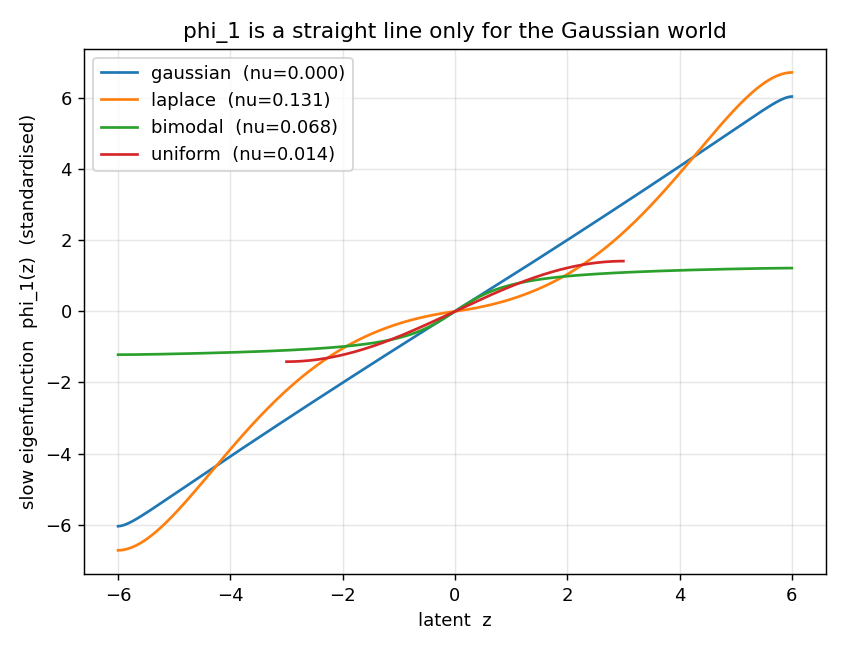
\includegraphics[width=0.78\linewidth,height=\textheight,keepaspectratio,alt={The recovered slow eigenfunction \textbackslash varphi\_1(z) is a straight line only for the Gaussian world; for every non-Gaussian law it is monotone but curved, by the nonlinearity \textbackslash nu = 1-R\^{}2 of its best affine fit (legend). This is the linear-versus-nonlinear identifiability boundary made visible: a linear probe of the representation is complete exactly where this curve is straight, and provably lossy in proportion to its bend.}]{empirical/apex_recovery/reports/e1_eigenfunctions.png}
\caption{The recovered slow eigenfunction \(\varphi_1(z)\) is a straight line \textbf{only} for the Gaussian world; for every non-Gaussian law it is monotone but curved, by the nonlinearity \(\nu = 1-R^2\) of its best affine fit (legend). This is the linear-versus-nonlinear identifiability boundary made visible: a linear probe of the representation is complete exactly where this curve is straight, and provably lossy in proportion to its bend.}
\end{figure}

\subsubsection{6.2 The bound, and the reality of the gap (E2)}\label{the-bound-and-the-reality-of-the-gap-e2}

On a product world we verify Theorem 3 directly. Across a sweep of leakage and whitening perturbations, the measured recovery error sits under \((\varepsilon+\sqrt{2\delta/\gamma})^2\) in \textbf{15 of 15} trials, with slack that stays of the order of the error (the bound is not vacuous) and vanishes at \(\delta=\varepsilon=0\). The product-spectrum check confirms (G): the two slowest joint modes are exactly the two single-coordinate slow modes (leakage \(0\) to machine precision), with \(\gamma=0.0224\). A deliberately heterogeneous pair (a fast and a slow coordinate) is shown to \emph{violate} (G) --- the slow coordinate's second mode outranks the fast coordinate's first --- and the certificate reports the guarantee as undefined there, exactly as it should. The gap is a checkable hypothesis, not a decoration.

\begin{figure}
\centering
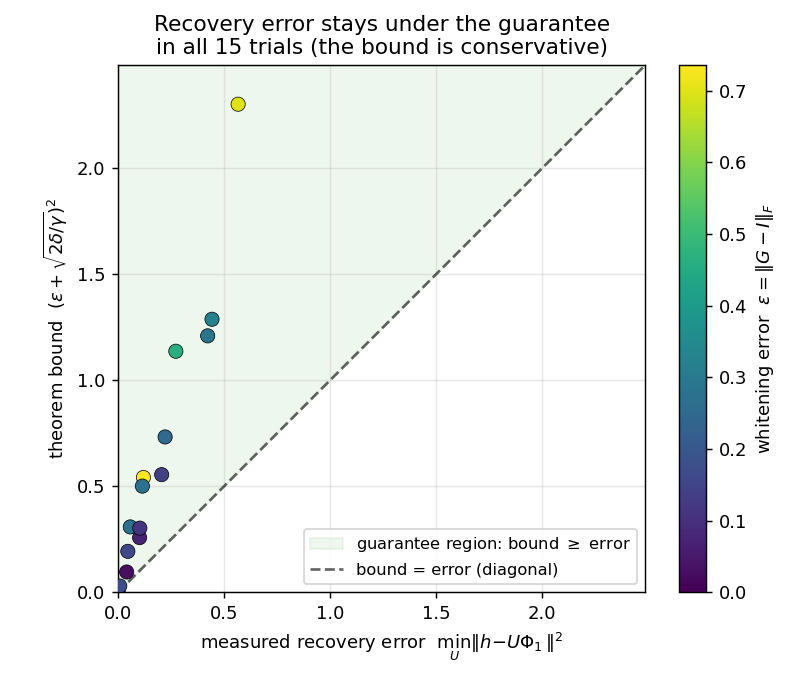
\includegraphics[width=0.52\linewidth,height=\textheight,keepaspectratio,alt={Approximate recovery (Theorem 3): across a sweep of whitening (\textbackslash varepsilon) and alignment (\textbackslash delta) perturbations, every measured recovery error \textbackslash min\_U\textbackslash\textbar h-U\textbackslash Phi\_1\textbackslash\textbar\^{}2 lies on or under the guarantee (\textbackslash varepsilon+\textbackslash sqrt\{2\textbackslash delta/\textbackslash gamma\})\^{}2 (dashed line; colour encodes \textbackslash varepsilon). The bound vanishes with the perturbations and is never vacuous.}]{empirical/apex_recovery/reports/e2_bound_scatter.png}
\caption{Approximate recovery (Theorem 3): across a sweep of whitening (\(\varepsilon\)) and alignment (\(\delta\)) perturbations, every measured recovery error \(\min_U\|h-U\Phi_1\|^2\) lies on or under the guarantee \((\varepsilon+\sqrt{2\delta/\gamma})^2\) (dashed line; colour encodes \(\varepsilon\)). The bound vanishes with the perturbations and is never vacuous.}
\end{figure}

\subsubsection{6.3 The finite register, and the blind-spot counts (E3)}\label{the-finite-register-and-the-blind-spot-counts-e3}

In exact rational arithmetic we exhibit the distributional tower of §3.4: a rank-three world's moment Hankel determinants are \(1,5,81,0\), closing at rank \(3\); the Prony/Hankel reconstruction recovers its levels \(\{-2,1,4\}\) exactly from the first six moments; and a two-level world is shown to be the affine (Gaussian-corner) case. The certificate then re-counts, from the distributional side, the cross-packet cubic triples of the cyclic head for \(n\in\{6,8,12,18,30\}\):
\[18,\quad 42,\quad 108,\quad 252,\quad 774,\]
\textbf{reproducing exactly} the conductor blind spot's published Section-4 counts. The same order-three object that the blind spot certifies finitely is the order-three rung whose continuous shadow bends \(\varphi_1\) in §6.1 --- the two registers, meeting on one set of integers.

\subsubsection{6.4 The bridge, measured (E4)}\label{the-bridge-measured-e4}

This certificate turns §3.4 from an argued correspondence into a measured one. Along a skew family interpolating from the Gaussian, the dynamical curvature \(\nu_D\) and the distributional skewness \(\tilde\kappa_3\) vanish together and rise locked by
\[\nu_D/\tilde\kappa_3^2 \;\longrightarrow\; 0.0555 \quad(\text{stable to }1.3\%\text{ across the near-Gaussian range}),\]
computed by Gauss--Hermite quadrature in the continuous (Ornstein--Uhlenbeck) limit, where the recovery map is exactly the inverse warp. Along a symmetric family the skewness is zero to machine precision (\(\sim 10^{-17}\)) while \(\nu_D/\tilde\kappa_4^2 \to 0.0104\) --- the recovery map still bends, but the first occupied rung is order four. The finite coda contrasts the two faces of order three: the cyclic label law has scalar skewness exactly zero, yet its Amari--Chentsov cross-packet cubic is nonzero (the counts of §6.3), so the structured index keeps order three alive where the scalar vanishes. We are explicit about what this does and does not establish: E4 measures the law in \textbf{two chosen one-parameter families} (a skew sweep and a symmetric sweep) and confirms the \textbf{leading-order} prediction \(\nu_D \propto (\text{leading cumulant})^2\) that §3.4 derives near the Gaussian. It does \emph{not} establish a universal quantitative relation between Amari--Chentsov cubic content and slow-eigenfunction curvature for arbitrary laws; it is the near-Gaussian law, measured where the theory says it should hold, not a global identity.

\begin{figure}
\centering
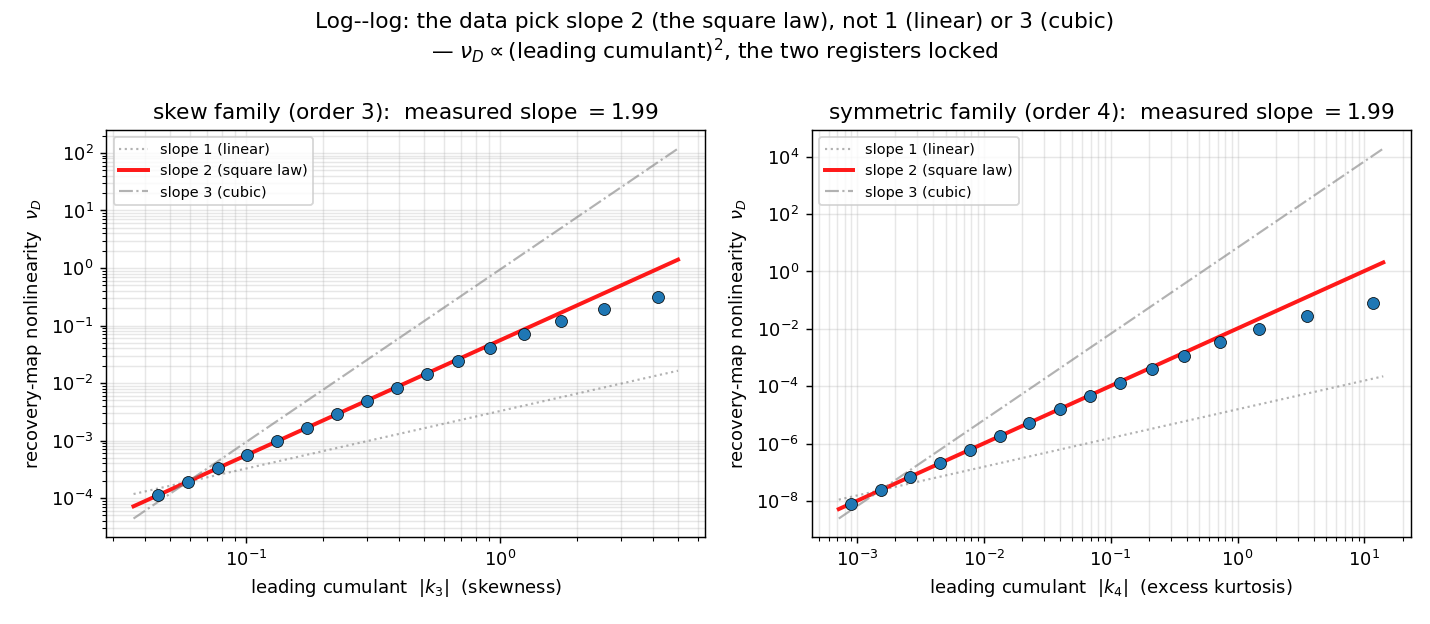
\includegraphics[width=0.92\linewidth,height=\textheight,keepaspectratio,alt={The cross-register bridge, measured. The recovery-map curvature \textbackslash nu\_D scales as the square of the leading distributional cumulant --- skewness\^{}2 for the skew family (left, order three) and excess-kurtosis\^{}2 for the symmetric family (right, order four) --- both vanishing with it at the Gaussian. The dashed line is the near-Gaussian slope; points fall below it at large departure (the square law is the leading-order statement).}]{empirical/apex_recovery/reports/e4_bridge.png}
\caption{The cross-register bridge, measured. The recovery-map curvature \(\nu_D\) scales as the square of the leading distributional cumulant --- skewness\(^2\) for the skew family (left, order three) and excess-kurtosis\(^2\) for the symmetric family (right, order four) --- both vanishing with it at the Gaussian. The dashed line is the near-Gaussian slope; points fall below it at large departure (the square law is the leading-order statement).}
\end{figure}

\subsubsection{6.5 On a real model: the bridge is a middle-layer phenomenon (E5)}\label{on-a-real-model-the-bridge-is-a-middle-layer-phenomenon-e5}

E4 is the continuous-limit twin of a question we can ask of an actual pretrained model: take the residual stream of a small language model (Pythia-70m), treat each coordinate of a layer as a ``world'', form positive pairs from adjacent token positions, estimate the slow eigenfunction of that token-to-token transition, and ask whether its curvature \(\nu_D\) tracks the coordinate's distributional cumulants. Two readings emerge, and we report both.

First, the \textbf{weak bridge} holds at every layer whose transition operator is estimable: the least non-Gaussian directions have near-floor curvature --- a Gaussian direction's recovery map is affine regardless of depth, the real-model image of §3.4's ``agree at the Gaussian corner.'' Second, the \textbf{strong} cross-direction link --- marginal non-Gaussianity predicting dynamical curvature across the 512 directions --- is \emph{not} uniform: it is a \textbf{middle-layer phenomenon}. The rank correlation between \(\nu_D\) and the leading-cumulant\(^2\) rises to \(+0.41\) at the centre of the network (layers 3--5) and is absent (\(\approx 0\)) at the embedding, the earliest, and the final layer. At the peak layer the two ends of the boundary are concrete: the most-Gaussian direction has an affine slow eigenfunction (\(\nu_D=0.03\)), while a heavy outlier dimension (skewness \(11.8\), excess kurtosis \(142\)) has a sharply curved one (\(\nu_D=0.51\)) --- a linear probe reads the first whole and the second only in part.

This depth dependence is exactly what the two-register picture predicts. The registers are \emph{distinct} objects off the Gaussian (§3.4); a coordinate can be skewed in its marginal yet affine in its slow dynamics if the non-Gaussianity lives in fast modes. They couple --- marginal shape showing up in the slow eigenfunction --- only where the slow dynamics carry the structure, which is the middle of the network, where representation is built, and not at the token-bound embedding or the output-shaped final layer. We do not force the clean E4 constant onto real activations; the depth profile, with its estimable-operator floor and its middle-layer peak, is the result. It is an observational certificate that sits \textbf{outside the theorem's hypotheses}, and we say so plainly: residual-stream coordinates are not independent latent factors; adjacent token positions are not a stationary, reversible, additive-noise transition; and \emph{symmetrising} the empirical adjacent-token operator imposes a reversibility the data need not have --- which risks partly \emph{manufacturing} the slow-eigenfunction object being measured rather than discovering it. We therefore read E5 as \textbf{suggestive corroboration} --- the predicted boundary is visible, unforced, in a pretrained network --- not as a test of the theorem. A construction that earns the assumptions (reversible pairs by design, factor-disentangled coordinates, an operator not symmetrised by hand) is the natural follow-up.

\begin{figure}
\centering
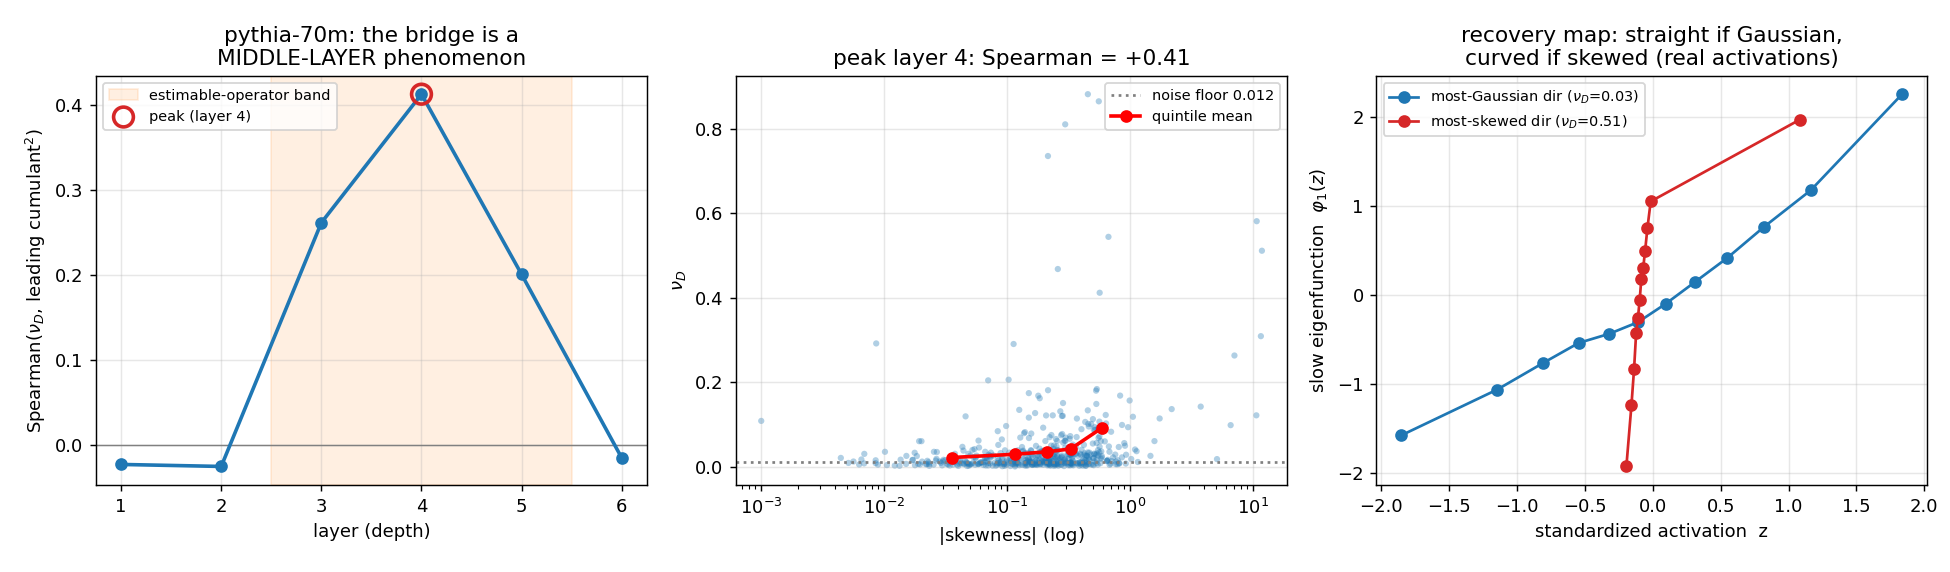
\includegraphics[width=1\linewidth,height=\textheight,keepaspectratio,alt={The bridge on a pretrained model (Pythia-70m). Left: the rank correlation between the slow-eigenfunction curvature \textbackslash nu\_D and the leading-cumulant\^{}2 across the 512 residual-stream directions is a middle-layer phenomenon, rising to +0.41 at the centre and vanishing at the embedding, earliest, and final layers. Centre: at the peak layer, \textbackslash nu\_D rises above the noise floor with \textbar skewness\textbar. Right: the two ends of the boundary --- a near-Gaussian direction has an affine recovery map (straight), a heavy outlier dimension a sharply curved one.}]{empirical/apex_recovery/reports/e5_real_model_bridge.png}
\caption{The bridge on a pretrained model (Pythia-70m). \emph{Left:} the rank correlation between the slow-eigenfunction curvature \(\nu_D\) and the leading-cumulant\(^2\) across the 512 residual-stream directions is a \textbf{middle-layer phenomenon}, rising to \(+0.41\) at the centre and vanishing at the embedding, earliest, and final layers. \emph{Centre:} at the peak layer, \(\nu_D\) rises above the noise floor with \(|\)skewness\(|\). \emph{Right:} the two ends of the boundary --- a near-Gaussian direction has an affine recovery map (straight), a heavy outlier dimension a sharply curved one.}
\end{figure}

\subsubsection{6.6 Planning: the chart is a faithful coordinate (E7)}\label{sec:e7}

The certificates so far test recovery and the bridge; this one tests §5 --- that the recovered chart is a faithful coordinate for \emph{control}. On a finite-horizon Markov decision problem whose latent reward is a narrow peak (so the optimal plan must localise the state precisely), the agent never sees the latent \(s\), only an observation \(o=g(s)\); its recovered chart is \(\psi=g^{-1}\), the slow-eigenfunction map E1 verifies --- affine on the Gaussian world, the cube-root on the non-Gaussian one. Everything is deterministic finite-horizon dynamic programming; three statements hold, exact where the theory is exact.

\textbf{Proposition 1, exact.} The \textbf{chart agent} --- which applies \(\psi\) to recover the true state, then plans --- matches the optimal return \(J^\star\) to machine precision (\(|J_{\text{chart}}-J^\star|<10^{-9}\)) on \emph{both} the Gaussian world and the nonlinear cube warp. Planning in the agent's own representation, with the change of variables applied, is exactly planning in the world --- for any diffeomorphism, Gaussian or not.

\textbf{The affine-iff-Gaussian boundary, in control.} The \textbf{linear agent} --- which reads the state off the observation with the best affine map, the control analogue of E1's linear probe --- is exact at the Gaussian corner (\(\nu=0\), regret \(0\)) and \textbf{silently sub-optimal off it}, its true-world regret climbing monotonically with the warp nonlinearity \(\nu\) (to \(\approx 63\%\) of the optimal return on the strongest warp tested). The boundary that makes a linear \emph{probe} incomplete makes a linear \emph{planner} sub-optimal; the remedy is the same recovered warp, applied now to the policy rather than the read-out.

\textbf{Theorem 4, certified.} With an imperfect chart of recovery RMS error \(\eta\), the chart agent's expected regret vanishes at \(\eta=0\) (recovering Proposition 1), grows \emph{linearly} in \(\eta\), and stays within \(C\,L\,T\,\eta\) with an \(O(1)\) constant (\(C\approx 0.03\) here; \(L\) the value Lipschitz constant, \(T\) the horizon). Planning degrades gracefully --- never catastrophically --- as recovery degrades.

\begin{figure}
\centering
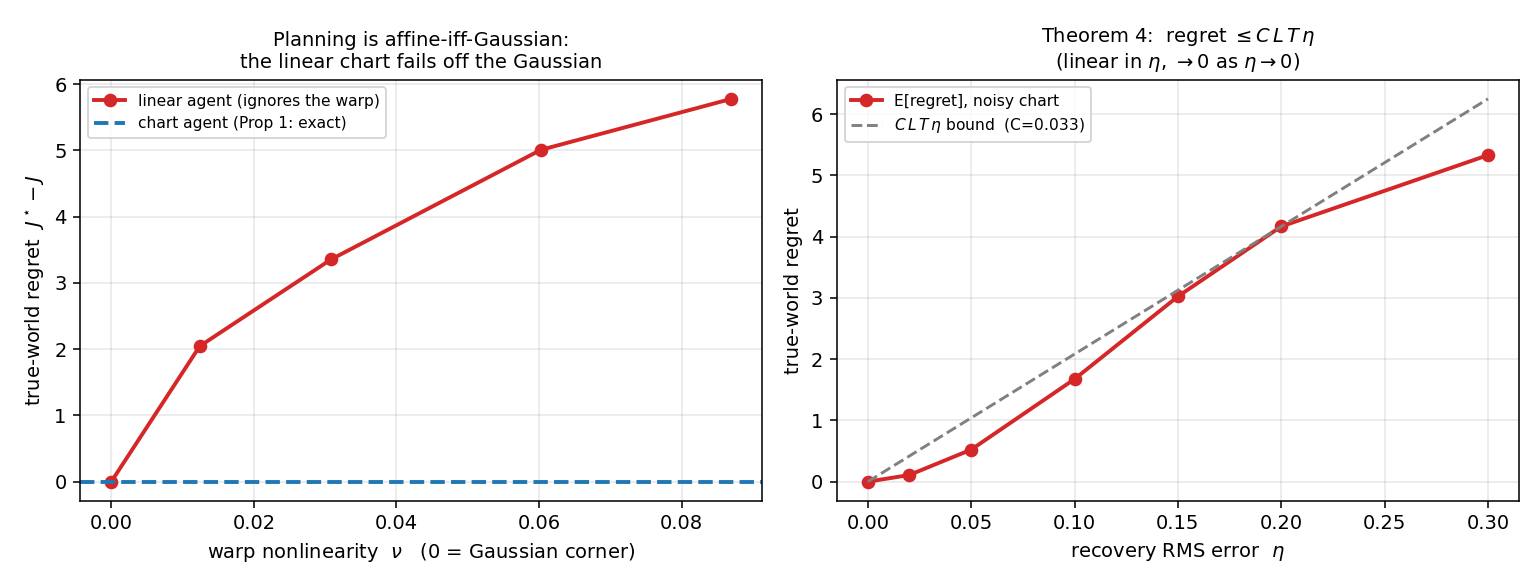
\includegraphics[width=0.92\linewidth,height=\textheight,keepaspectratio,alt={Planning is faithful when the chart is applied, and only affine-when-Gaussian when it is not. Left: the linear agent's true-world regret climbs from zero at the Gaussian corner with the warp nonlinearity \textbackslash nu, while the chart agent (Proposition 1) stays exact. Right: with a noisy chart, the chart agent's regret is linear in the recovery error \textbackslash eta and stays under the C\textbackslash,L\textbackslash,T\textbackslash,\textbackslash eta bound of Theorem 4, vanishing as \textbackslash eta\textbackslash to 0.}]{empirical/apex_recovery/reports/e7_planning.png}
\caption{Planning is faithful when the chart is applied, and only affine-when-Gaussian when it is not. \emph{Left:} the linear agent's true-world regret climbs from zero at the Gaussian corner with the warp nonlinearity \(\nu\), while the chart agent (Proposition 1) stays exact. \emph{Right:} with a noisy chart, the chart agent's regret is linear in the recovery error \(\eta\) and stays under the \(C\,L\,T\,\eta\) bound of Theorem 4, vanishing as \(\eta\to 0\).}
\end{figure}

\subsubsection{6.7 The encoder reaches the optimum by training (E8)}\label{sec:e8}

Theorem 1 identifies the alignment-and-whitening \emph{population optimum} as the slow-eigenfunction chart, and the certificates above verify that optimum as an eigenproblem. They leave one gap a careful reader will press: does a \emph{gradient-trained} encoder actually reach it? This certificate closes it by training rather than solving. A small encoder is trained by SGD on the self-supervised objective --- alignment of temporally adjacent pairs plus a VICReg whitening penalty --- reading only a fixed, high-dimensional, \emph{nonlinear} observation of the latent (random Fourier features); it is never handed \(z\) or \(\varphi_1\).

It reaches the chart. On four worlds --- a Gaussian and three non-Gaussian --- the trained encoder recovers \(\varphi_1\) with \(\pi\)-weighted correlation \(0.96\) (Gaussian), \(0.99\) (Laplace), and \(0.999\) (bimodal, uniform), and the recovered map's nonlinearity tracks the target's: the red trained chart lies on the blue eigenfunction through the bulk of every world. So for one-dimensional recovery the gap between the population optimum and what SGD reaches is small. We are precise about what blurs and what holds: a trained MLP carries its own \(\sim\!0.06\) curvature floor, so it does \emph{not} sharply resolve the affine-iff-Gaussian boundary among the \emph{mild} worlds --- the analytic certificate E1 owns that clean statement --- and what E8 adds is the harder, more practical fact that \emph{training finds the chart at all}.

The multi-dimensional case is honestly harder, and we report it rather than tune it away. On a two-dimensional product world a 2-D head with the full whitening term whitens correctly --- its embedding Gram is the identity --- but reaches the joint top-two slow subspace only \emph{partially}: one mode cleanly, the other to about \(65\%\) (Procrustes error \(\approx 0.7\)). So the population-vs-trained gap, negligible for the one-dimensional optima, is real and larger for the block rotation: training reliably reaches each factor's chart; aligning the full rotation is the part SGD leaves on the table here.

\begin{figure}
\centering
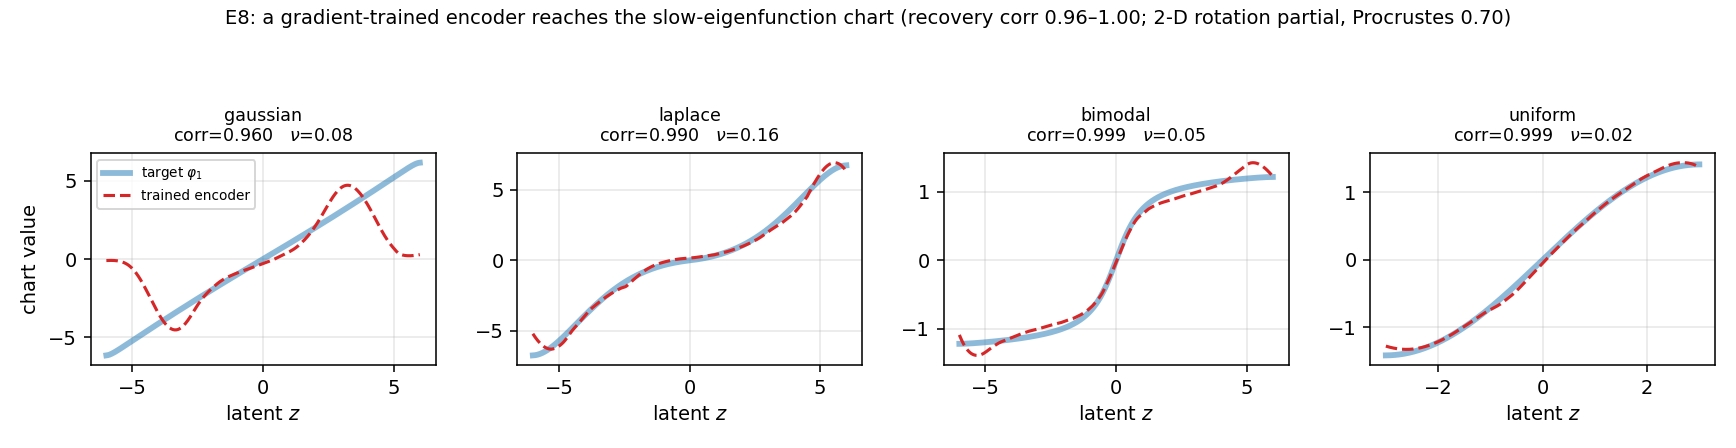
\includegraphics[width=1\linewidth,height=\textheight,keepaspectratio,alt={A gradient-trained encoder reaches the slow-eigenfunction chart. For each world the recovered chart (red, sign- and scale-aligned for display) lies on the target \textbackslash varphi\_1 (blue) through the bulk of the stationary mass; the Gaussian's tail wiggle is the unconstrained region where \textbackslash pi\textbackslash approx 0. Recovery correlations are 0.96--1.00; the two-dimensional rotation is recovered only partially (Procrustes 0.70), an honestly reported limitation.}]{empirical/apex_recovery/reports/e8_trained_encoder.png}
\caption{A gradient-trained encoder reaches the slow-eigenfunction chart. For each world the recovered chart (red, sign- and scale-aligned for display) lies on the target \(\varphi_1\) (blue) through the bulk of the stationary mass; the Gaussian's tail wiggle is the unconstrained region where \(\pi\approx 0\). Recovery correlations are \(0.96\)--\(1.00\); the two-dimensional rotation is recovered only partially (Procrustes \(0.70\)), an honestly reported limitation.}
\end{figure}

\begin{center}\rule{0.5\linewidth}{0.5pt}\end{center}

\subsection{7. Consequences for practice}\label{sec:consequences}

The dichotomy is not only structural; it has operational teeth for how learned representations are read, trained, and trusted.

\textbf{Interpretability and explainability.} Linear probing is the default instrument for asking what a representation encodes. Theorem 2 says that instrument is \emph{complete only on the Gaussian stratum}: wherever the underlying factors are non-Gaussian --- which is to say, wherever the world has genuine higher-order structure --- a linear probe reads a strict shadow of what the representation has identified, and the missing part is precisely the curvature of \(\varphi_1\). The remedy is not a bigger probe but the \emph{right} one: the recovered chart is nonlinear and recoverable (by operator/cumulant estimation, §3.3), so a probe matched to \(\Phi_1\) recovers what a linear probe cannot. This is suggested in a pretrained model (§6.5): at the middle layers, the most non-Gaussian residual-stream directions --- the heavy outlier dimensions known to dominate transformer activations --- \emph{tend} to be the ones whose recovered slow feature is curved, so a linear read of them is partial. This also explains, without appeal to optimization pathology, why linear-probe audits can under-report capability on structured tasks.

\textbf{Optimization --- and a distinction that matters.} It is tempting to read this as ``second-order methods have a ceiling,'' but that would conflate three different things called \emph{second-order}, and only two of them are limited. (a) A linear \emph{readout} of the representation is order-one and is complete only on the Gaussian stratum (§3.2). (b) A second-order \emph{curvature model} --- the Fisher / Gauss--Newton / K-FAC class, which represents the loss curvature as a quadratic form --- is matched to the Gaussian corner and cannot carry the order-three content; that is the conductor blind spot's own statement, and it is the same distributional cubic. But (c) an \emph{objective} that merely uses second moments is \textbf{not} so limited: our own alignment-and-whitening objective imposes a second-moment (whitening) constraint yet, minimised over a nonlinear encoder, recovers the \emph{fully nonlinear} slow-eigenfunction chart at its population optimum. So the ceiling is in the linear readout and the quadratic curvature \emph{model}, not in second-order \emph{training} as such --- the failure a practitioner meets is in the linear read of the result, not in using covariances to learn it. The constructive corollary is unchanged: the gap \(\gamma\) is an estimable diagnostic of \emph{how well-posed} slow-feature recovery is for a given encoder and task, and a small \(\gamma\) is an early warning that the representation's slow structure is nearly degenerate.

\textbf{Auditing and the governance of world models.} Identifiability is the property a regulator or safety auditor most wants from a learned world model: that the representation corresponds to the world's real degrees of freedom rather than scrambling them. This paper sharpens what can be promised. Identifiability \emph{does} hold for non-Gaussian worlds --- the representation recovers the true factors --- but only \textbf{up to a recoverable nonlinear chart and a block rotation}, and only when the slow-feature gap (G) holds. An audit that assumes \emph{linear} correspondence will mis-certify a perfectly identified non-Gaussian representation as entangled; an audit that checks the \emph{gap} and reconstructs the \emph{chart} (an explicit estimation step, not a free read of the encoder) will not. The planning theorem makes the stakes concrete: a controller that plans in the representation acts in the world exactly, provided the recovered warp is applied --- and silently sub-optimally if it is assumed away.

\textbf{Anisotropy as a design lever.} Theorem 1's fine print is an opportunity: distinct mixing rates across factors turn the rotation ambiguity into per-coordinate identification. A learner or augmentation scheme that \emph{induces} anisotropy buys disentanglement without an auxiliary objective --- a direction we flag for separate study.

\textbf{Spectral-gap engineering.} The same theory makes augmentation design quantitative rather than intuitive. Positive pairs are not ``added noise''; they \emph{define} the transition operator \(T\), and what the encoder keeps is decided entirely by \(T\)'s spectrum (Theorem 1) with well-posedness governed by the gap (G) (Theorem 3). The lever a practitioner actually holds is therefore the gap \(\gamma\): a factor is retained iff its mixing rate places it among the slowest \(n\) modes, and the recovery is robust in proportion to how far it sits above the fastest discarded mode --- a nuisance's leakage into the representation is bounded by \(\delta/\gamma\) (§4). Two consequences follow. First, to make a representation \emph{ignore} a nuisance, design the augmentation so that factor mixes \emph{fast} (small \(\lambda\), placed below the retained band) --- not by penalising it downstream but by demoting it in the spectrum. Second, and unlike most design choices, \(\gamma\) is \emph{computable from the augmentation kernel before any training}: one can certify in advance that the invariances the optimum will learn are the ones intended. The gap is, in effect, a pre-registration of what an SSL pipeline will and will not encode.

\textbf{Grokking: the prediction, now tested.} The sharpest forward use of the two-register picture is dynamical, and we have run it. On the canonical delayed-generalisation task --- modular addition \(a+b\equiv c \pmod n\) --- the generalising ``Fourier circuit'' is an order-three object: it computes via the character selection rule \(k+\ell+m\equiv 0\pmod n\), the same Amari--Chentsov cubic the conductor blind spot names, while the memorising solution that precedes it is order-two-sufficient (a lookup with no ring structure). Grokking should then be the order-two \(\to\) order-three boundary of this paper \emph{crossed during training}: at the generalisation step the distributional register (the head becoming ring-additive, depending on \(a+b\) alone) and the dynamical register (the token embedding circularising onto its slow-eigenfunction character chart) should rise \textbf{together}, both tracking validation accuracy and both flat on a structure-free control. Training a one-layer transformer to the grok confirms exactly this, on a prime modulus (\(p=113\), generalisation at step \(18{,}000\)) and on a composite one (\(n=110\), step \(35{,}000\)): embedding Fourier concentration and head additivity climb together through the transition to validation accuracy one, while a matched random-table control stays flat in every register. The strong falsifier held --- the two registers did \emph{not} rise at different times.

Two honest qualifications attach to the cross-packet \emph{refinement} of this picture. First, the blind spot's literal diagnostic --- the cross-packet mass of the centered score --- does \textbf{not} transfer to this task: a generalised modular-addition head outputs a near-delta, so its score-cubic \emph{vanishes} as the model becomes correct (its total mass collapses by many orders of magnitude through the grok) and it does not separate ring from control. The ring structure lives in the input→output \emph{map}, which the two registers read, not in the marginal output's score-cubic. Second, a \emph{persistent} form of the same diagnostic --- the cross-packet cubic of the logits' offset profile, which \emph{grows} rather than vanishes as the model generalises --- does separate cleanly. On both a composite modulus (\(n=110\)) and a prime-power one (\(n=121=11^2\), which has a single packet-difference set), the \textbf{absolute cross-packet mass} accumulates on the ring task during the representation-learning phase, peaking three-to-five orders of magnitude above the structure-free control, which holds the baseline throughout. This is precisely the directional behaviour the conductor blind spot's trajectory conjecture predicts --- cross-packet activation accumulating on a ring task and staying null on a matched label-permuted control --- and it matches that conjecture's depth-driven refinement specifically: the accumulation is a representation-learning-phase phenomenon, building \emph{before} the generalisation step, and on the prime-power modulus it consolidates \emph{within} a packet once the solution finalises (the cross-packet \emph{share} falls toward zero post-grok even as the total cubic mass explodes). We are precise about scope: the measurement is on the head's logit offset profile --- a persistent transform that reflects the trained upstream features rather than the categorical head in isolation, consistent with that same refinement --- so this is trajectory evidence in the predicted direction, not a from-scratch proof of the conjecture's mechanism.

We keep the epistemic status exact: this is a \emph{prediction tested, not a consequence proven}. Nothing in §§3--5 derives that modular-addition grokking is an order-two→order-three transition; the theory supplies only the order-three identity of the generalising circuit and the co-emergence hypothesis, and the experiment adjudicates --- finding, on two moduli, the co-emergence the picture requires, and keeping the cross-packet diagnostic's reach honestly bounded.

\begin{center}\rule{0.5\linewidth}{0.5pt}\end{center}

\subsection{8. Scope and limitations}\label{sec:scope}

The theorems are conditional and we state the conditions plainly. \textbf{Reversibility} (detailed balance) buys the self-adjoint spectral theorem; for genuinely non-reversible additive noise a companion note proves that the single-encoder objective sees only the symmetric part \(\tfrac12(T+T^{*})\) and is \emph{exactly} blind to the antisymmetric current --- the arrow of time --- a sibling blind spot on the reversibility axis (orthogonal to this paper's cumulant axis), resolved by a predictive two-encoder objective and certified deterministically on the drift ring. \textbf{Product (independent-factor) structure} of the latent law is assumed throughout (§2.2): it is what makes the eigenfunctions of \(T=\bigotimes_iT_i\) factor into single-coordinate modes, so that under (G) the \(n\) slowest joint modes are the \(n\) per-coordinate leaders \(\varphi_1^{(i)}\) (Theorem 1, Appendix A.2). Correlated or non-factorising latents break this single-excitation accounting --- the recovered object is then the joint slow eigenspace rather than a coordinatewise warp --- and are likewise left to follow-up. \textbf{Discrete spectrum} (compact \(T_i\)) holds for Ornstein--Uhlenbeck and confining Langevin generators; heavy-tailed or unconfined laws may add continuous spectrum. The \textbf{slow-feature gap (G)} is a real hypothesis, checkable and sometimes false (§6.2). Recovery is \textbf{up to a nonlinear chart}: this is the correct and honest statement, not a weakness --- claiming linear recovery off the Gaussian would be false. Theorem 4 (approximate planning) assumes \textbf{Lipschitz value functions and a bi-Lipschitz chart}; its constant, given in Appendix A.6, carries the chart's bi-Lipschitz modulus and is finite away from the support boundary. Finally, the bridge of §3.4 is a statement about \emph{model classes and registers}, not a claim that a single diagnostic has been run end-to-end across both; §6 checks each register on its own ground, and the cross-register experiment flagged in the internal log is the natural next step.

\textbf{Empirical scope.} The certificates are deliberately small and exact rather than large and benchmarked, and we are plain about the ceiling that leaves. The deterministic certificates (E1--E4, E7) and the trained-encoder certificate (E8) run on \emph{synthetic} one- and two-dimensional worlds with known ground-truth warps and random-Fourier observations; we have \emph{not} tested recovery on a large-scale real self-supervised benchmark --- images, video, audio --- with independently known non-Gaussian factors, and the per-factor-versus-block-rotation gap that E8 already measures in two dimensions (§6.7) is the kind of effect that may widen with dimension. The single real-model certificate (E5) is observational, on one small language model, and sits outside the theorem's hypotheses (§6.5); we read it as suggestive corroboration, not a test. The grokking measurement (§7) is on a \emph{one-layer} transformer at two moduli, and its cross-packet \emph{refinement} is trajectory evidence in the predicted direction --- co-emergence of the two registers, with a persistent cross-packet diagnostic that accumulates on the ring task and stays null on the matched control --- not a from-scratch mechanistic proof of the trajectory conjecture. The three principal empirical follow-ups are therefore: a large-scale real-SSL test with known non-Gaussian factors; a multi-layer, multi-model, multi-architecture grokking study; and a construction that \emph{earns} E5's reversibility-and-disentanglement assumptions by design (reversible pairs, factor-disentangled coordinates, an operator not symmetrised by hand) rather than imposing them on activations.

\begin{center}\rule{0.5\linewidth}{0.5pt}\end{center}

\subsection{9. Conclusion}\label{sec:conclusion}

The conductor blind spot showed, on a clock, that an order-two instrument cannot read an order-three fact. This paper showed the corresponding boundary in the continuous, learned setting: the alignment-and-whitening \emph{optimum} recovers the slow-eigenfunction chart of a world; that chart is a straight line exactly for the Gaussian (in the observed coordinate) and a recoverable curve otherwise; recovery is exact up to a block rotation, robust by a gap-controlled bound, and faithful for planning under a recoverable change of variables. The Gaussian corner --- where a linear probe is complete and the warp is the identity --- is one stratum of a theory whose general statement is nonlinear, and whose limits and licenses we have tried to state without flinching. The finite and the continuous, the distributional and the dynamical, meet on the same integers; the practical lesson is to read a representation through the chart it actually learned, and to certify the gap that makes that chart well-posed.

\begin{center}\rule{0.5\linewidth}{0.5pt}\end{center}

\subsection{Appendix A. Proofs}\label{sec:appA}

\subsubsection{A.1 Alignment as a Rayleigh form}\label{sec:A1}

With \(\{h_i\}\) whitened and \(T\) self-adjoint, stationarity gives \(\mathbb E[h_i(z)^2]=\mathbb E[h_i(z')^2]=1\) and, by the definition of \(T\) as conditional expectation, \(\mathbb E[h_i(z')h_i(z)] = \mathbb E[h_i(z)\,\mathbb E[h_i(z')\mid z]] = \langle h_i, Th_i\rangle\). Hence
\[\mathbb E\|h(z')-h(z)\|^2 = \sum_i\big(\mathbb E[h_i(z')^2]+\mathbb E[h_i(z)^2]-2\mathbb E[h_i(z')h_i(z)]\big) = \sum_i 2\big(1-\langle h_i,Th_i\rangle\big).\qquad\square\]

\subsubsection{A.2 Ky Fan and the product spectrum}\label{sec:A2}

\emph{Ky Fan maximum principle.} For self-adjoint compact \(T\) and orthonormal \(\{h_i\}_{i=1}^n\) in the mean-zero subspace, \(\max\sum_i\langle h_i,Th_i\rangle\) equals the sum of the \(n\) largest non-trivial eigenvalues of \(T\), attained iff \(\mathrm{span}\{h_i\}\) is the corresponding top eigenspace; the maximiser is unique up to orthogonal mixing within degenerate blocks (Fan 1949).

\emph{Product spectrum.} The spectrum of \(T=\bigotimes_iT_i\) is \(\{\prod_i\lambda_{k_i}^{(i)}\}\) with eigenfunctions \(\bigotimes_i\varphi_{k_i}^{(i)}\). Under (G), the \(n\) largest non-trivial eigenvalues are the single-excitations \(\{\lambda_1^{(i)}\}\) with eigenfunctions \(\varphi_1^{(i)}(z_i)\): any competitor is a higher single mode (\(\le\lambda_2^{(i)}\)) or a multi-excitation (\(\le\lambda_1^{(i)}\lambda_1^{(j)}\)), both strictly dominated by (G). Combining with Ky Fan gives Theorem 1, with the equal-\(\lambda_1\) degeneracy as the only freedom in \(U\). \(\square\)

\subsubsection{A.3 Affine recovery iff Gaussian}\label{sec:A3}

We work in the reversible \textbf{diffusion} realisation \(T_i=e^{\tau L_i}\) with \(L_i\psi = D(\psi''+(\log p_i)'\psi')\), whose eigenfunctions are those of \(T_i\) (this is the load-bearing hypothesis: a general reversible kernel of §2.2 need not have this generator). If \(\varphi_1(z)=az+b\) (\(a\ne 0\)), then \(L_i\varphi_1 = aD(\log p_i)'\), and \(L_i\varphi_1=-\mu\varphi_1\) forces \((\log p_i)'(z) = -\tfrac{\mu}{aD}(z+b/a)\), so \(\log p_i\) is quadratic. \textbf{Under full support on \(\mathbb R\) and natural (no-flux) boundary conditions}, the only normalisable quadratic-log density is the Gaussian, and \(\mu>0\) fixes the sign --- giving \(p_i\) Gaussian. On a bounded interval, a finite grid, or with reflecting/non-natural boundary conditions this last step fails: the boundary terms re-enter the Sturm--Liouville problem, and an affine first eigenfunction can occur for non-Gaussian \(p_i\) (the finite symmetric case of §3.3 is the minimal counterexample). This is exactly why Theorem 2 is a full-support, natural-boundary statement. Conversely the Gaussian gives Ornstein--Uhlenbeck, whose first eigenfunction is \(\varphi_1(z)=z\). \(\square\)

\subsubsection{A.4 Finite rank and Hankel reconstruction (restated in-house)}\label{sec:A4}

Let a coordinate take \(r\) distinct values \(\lambda_1,\dots,\lambda_r\) with weights \(w_j>0\), \(\sum w_j=1\), and write \(\mu_k=\sum_j w_j\lambda_j^k\).

\textbf{(Rank closure.)} The Hankel matrices \(H_N=[\mu_{a+b}]_{0\le a,b\le N}\) satisfy \(\det H_N>0\) for \(N<r\) and \(\det H_r=0\): the moment sequence has exact rank \(r\). (Standard for an \(r\)-atomic measure; the positive-definiteness is Hamburger's condition.)

\textbf{(Reconstruction.)} The levels are the roots of the degree-\(r\) Prony polynomial whose coefficients solve the Hankel system \([\mu_{a+b}]_{0\le a,b<r}\,c = -[\mu_r,\dots,\mu_{2r-1}]^\top\); the weights then solve a Vandermonde system. Hence \(r\) levels and weights are determined by \(\mu_0,\dots,\mu_{2r-1}\) --- the first \(2r\) moments. \(\square\)

This is the \emph{distributional} tower (§3.4): the orthogonal polynomials of \(p_i\) are fixed by the same Hankel data and form a tridiagonal (Jacobi) recurrence. It reconstructs the \textbf{world's law and effective rank}, not the transition eigenfunction; the two coincide only at the Gaussian.

\subsubsection{A.5 The approximate bound (trace-gap Davis--Kahan)}\label{sec:A5}

Work with \(A=I-T\) on the mean-zero subspace, eigenvalues \(a_k=1-\lambda_k\); let \(V_n\) be the bottom-\(n\) eigenspace (top-\(n\) of \(T\)), \(P\) its projector, and \(\theta^2=\|P^\perp\Pi_W\|_{HS}^2\) the leakage of \(W=\mathrm{span}(\tilde h)\) out of \(V_n\). The gap is \(\gamma=a_{n+1}-a_n\).

\textbf{Lemma (trace-gap).} \(\mathrm{tr}(A\Pi_W)\ge \sum_{i\le n}a_i + \gamma\theta^2\).

\emph{Proof.} Split \(\tilde h_i=u_i+v_i\), \(u_i=P\tilde h_i\). The discarded part gives \(\sum_i\langle v_i,Av_i\rangle\ge a_{n+1}\theta^2\). For the retained part, \(\Sigma=P\Pi_WP\) satisfies \(0\preceq\Sigma\preceq I_{V_n}\), \(\mathrm{tr}\Sigma=n-\theta^2\), and minimising \(\mathrm{tr}(A|_{V_n}\Sigma)\) fills the smallest eigenvalues: \(\sum_i\langle u_i,Au_i\rangle\ge\sum_{i\le n}a_i - a_n\theta^2\). Add and use \(a_{n+1}-a_n\ge\gamma\). \(\square\)

Approximate alignment (\(\mathrm{tr}(A\Pi_W)\le\sum_{i\le n}a_i+\delta\)) then gives \(\theta^2\le\delta/\gamma\). An orthogonal-Procrustes step (with \(C_{ij}=\langle\tilde h_i,\varphi_1^{(j)}\rangle\): the \(\tilde h_i\) are orthonormal and the \(\varphi_1^{(j)}\) orthonormal, so \(C\) is a sub-block of an orthogonal matrix with singular values \(\le 1\) and \(\sum_k\sigma_k^2 = n-\theta^2\); thus \(\min_U\|C-U\|_F^2 = \sum_k(1-\sigma_k)^2 \le \sum_k(1-\sigma_k^2)=\theta^2\)) yields \(\min_U\|\tilde h-U\Phi_1\|^2 \le \theta^2 + \theta^2 = 2\theta^2 \le 2\delta/\gamma\).

Finally we account for inexact whitening, spelling out the norm bookkeeping. The Gram \(G_{ij}=\langle h_i,h_j\rangle\) is symmetric positive-definite; diagonalise \(G=Q\,\mathrm{diag}(g_k)\,Q^\top\) with \(g_k>0\). The whitened encoder is \(\tilde h = G^{-1/2}h\), so \(h-\tilde h = (I-G^{-1/2})h\) and, since \(\langle h_i,h_j\rangle=G_{ij}\),
\[\|h-\tilde h\|_{L^2(p)}^2 = \mathrm{tr}\!\big((I-G^{-1/2})\,G\,(I-G^{-1/2})\big) = \sum_k\big(\sqrt{g_k}-1\big)^2 .\]
Because \((\sqrt{g_k}-1)^2 = (g_k-1)^2/(\sqrt{g_k}+1)^2 \le (g_k-1)^2\), and \(\sum_k(g_k-1)^2 = \|G-I\|_F^2 \le \varepsilon^2\) (the Frobenius norm is the sum of squared eigenvalue deviations and is unitarily invariant), we obtain \(\|h-\tilde h\|\le\varepsilon\). The triangle inequality \(\min_U\|h-U\Phi_1\| \le \|h-\tilde h\| + \min_U\|\tilde h-U\Phi_1\| \le \varepsilon+\sqrt{2\delta/\gamma}\), squared, is the claim. \(\square\)

\subsubsection{A.6 Planning equivalence}\label{sec:A6}

\textbf{Proposition 1 (exact).} Backward induction on \(t\). Base: \(\widehat V^\star_T(\psi(z))=\widehat c_T(\psi(z))=c_T(z)=V^\star_T(z)\). Step: assume \(\widehat V^\star_{t+1}(\psi(z'))=V^\star_{t+1}(z')\). By the pushforward identity \(\int g(\widehat z')\widehat P_t(d\widehat z'\mid\psi(z),a)=\int g(\psi(z'))P_t(dz'\mid z,a)\) with \(g=\widehat V^\star_{t+1}\), and \(\widehat c_t(\psi(z),a)=c_t(z,a)\),
\[\widehat V^\star_t(\psi(z)) = \min_a\Big\{c_t(z,a)+\int V^\star_{t+1}(z')P_t(dz'\mid z,a)\Big\} = V^\star_t(z),\]
with identical minimands in \(a\), so the optimal actions coincide. The native- and invariant-cost corollaries are immediate: if the objective is given on \(\widehat z\) no \(\psi\) is needed; if \(c\circ\psi^{-1}=c\) it is evaluated on \(\widehat z\) directly, reducing at \(\Phi_1=\mathrm{id}\) to rotation-invariance. \(\square\)

\textbf{Theorem 4 (approximate).} The agent decodes its observation to a believed latent \(\tilde z := \psi^{-1}(h(z))\) and executes the action \(a^\star_t(\tilde z)\) optimal at \(\tilde z\). With \(\psi\) bi-Lipschitz, \(\|\psi^{-1}(u)-\psi^{-1}(v)\|\le\kappa\|u-v\|\), so the state-decoding error obeys, by Cauchy--Schwarz and the Theorem 3 bound,
\[\mathbb E\|\tilde z - z\| = \mathbb E\big\|\psi^{-1}(h(z))-\psi^{-1}(\psi(z))\big\| \le \kappa\,\mathbb E\|h(z)-\psi(z)\| \le \kappa\big(\mathbb E\|h-\psi\|^2\big)^{1/2} \le \kappa\,\eta.\]
By the performance-difference lemma (Kakade--Langford 2002), the regret of executing, at each step, the action optimal for a state estimate that is off by \(\Delta_t\) is at most \(2\sum_{t} \mathrm{Lip}(V^\star_t)\,\mathbb E\|\tilde z_t - z_t\|\). Here \textbf{transition stability} earns its place: because the kernels \(P_t(\cdot\mid z,a)\) are Lipschitz in the state, the believed and the true trajectories evolve under nearby kernels, so the per-step decoding error stays \(O(\kappa\eta)\) along the executed path rather than compounding step-to-step --- without this, a small initial misidentification could amplify and the sum would not be controlled. With each \(V^\star_t\) \(L\)-Lipschitz and the per-step decoding error thus \(\le\kappa\eta\) over horizon \(T\),
\[\mathbb E\big[V^{\hat\pi}_0(z)-V^\star_0(z)\big] \le 2\kappa\,L\,T\,\eta =: C\,L\,T\,\eta .\]
At \(\eta=0\) the bound is zero and \(\tilde z=z\), recovering Proposition 1. \(\square\)

\emph{Remark.} The constant \(C=2\kappa\) carries the chart's bi-Lipschitz modulus, which is finite wherever the stationary density is bounded away from \(0\) on the planning region (so \(\varphi_1^{(i)}\) has positive, bounded derivative there); the bound is vacuous only as that region approaches a support boundary, exactly where the chart itself degenerates.

\begin{center}\rule{0.5\linewidth}{0.5pt}\end{center}

\subsection{Appendix B. The conductor blind spot as the finite, distributional register}\label{sec:appB}

We make §3.4 explicit. The conductor blind spot studies the categorical model at the uniform point \(p_*\) on \(\mathbb Z/n\mathbb Z\): the Fisher form is diagonal in the additive-character basis, block-diagonal across conductor packets, while the Amari--Chentsov cubic couples packets under \(k+\ell+m\equiv 0\pmod n\). These are statements about the \textbf{stationary law's} local geometry --- the distributional tower --- read at order two and order three.

The present paper's recovery map is the \textbf{dynamical} slow eigenfunction. At the Gaussian/uniform corner the two towers coincide (Hermite simultaneously diagonalises the Ornstein--Uhlenbeck transition and orthogonalises the Gaussian), and the degree-\(d\) rung carries transition eigenvalue \(\rho^d\); the order-three cubic is then the degree-three eigenspace, eigenvalue \(\rho^3\), the first rung below the recovered degree-one mode. Off the corner the towers split: the cubic remains a distributional order-three object, while the dynamical \(\varphi_1\) becomes a mixture of distributional orders and bends.

The certificate of §6.3 lives entirely on the distributional side and regenerates the blind spot's cross-packet cubic counts \(18,42,108,252,774\) for \(n\in\{6,8,12,18,30\}\), confirming that the order-three object this paper's continuous theory points to is, on the finite cyclic index, exactly the one the blind spot certifies. The two papers therefore share an order-three witness: finite and exact there, continuous and learned here.

\textbf{Scalar versus tensor: why the ring is special.} One subtlety is worth stating plainly, because the measured bridge of §6.4 exposes it. The order-three content of an \emph{unstructured} one-dimensional world is the scalar third cumulant (the skewness), and it vanishes whenever the law is symmetric --- there the recovery map first bends at order four. The conductor blind spot's order-three object is not a scalar but the Amari--Chentsov \emph{tensor} on the tangent space, and its cross-packet components are nonzero at the symmetric maximum-entropy point precisely because the cyclic index supplies the arithmetic that survives the symmetry (the selection rule \(k+\ell+m\equiv 0\pmod n\) has solutions with unequal conductors). So the ring structure is exactly what keeps order three occupied where a scalar skewness would be silent. This is not a discrepancy between the registers; it is the reason the blind spot is an order-three statement at \(p_*\) at all, and it is measured directly in §6.4 (scalar skewness zero, tensor cubic nonzero, on the same \(n\)).

\begin{center}\rule{0.5\linewidth}{0.5pt}\end{center}

\subsection{Appendix C. Experimental protocol and reproduction}\label{sec:appC}

All code lives in \href{https://github.com/leomurillo/AI-ConductorBlindSpot/tree/main/empirical/apex_recovery}{\texttt{empirical/apex\_recovery/}} of the companion repository; running \href{https://github.com/leomurillo/AI-ConductorBlindSpot/blob/main/empirical/apex_recovery/run_all.py}{\texttt{run\_all.py}} there reproduces every number (use the figure-capable interpreter to also render the \texttt{.png} figures). The runner asserts the headline self-checks --- the approximate bound holds in every trial; the finite reconstructions are exact; the blind-spot counts match; the cross-register square law is stable and positive; the planning chart agent is exact and its Theorem-4 regret bound holds --- and exits nonzero on any failure.

\textbf{Worlds.} Each world is a reversible nearest-neighbour Metropolis chain on a grid --- the exact, fully diagonalisable discrete counterpart of the Ornstein--Uhlenbeck transition. The transition operator is symmetrised in the \(\pi\)-weighted inner product and diagonalised by a symmetric eigensolver; eigenfunctions are \(L^2(p)\)-orthonormal. There is no randomness in the operators; the only seed is the contamination sweep of E2.

\textbf{E1} (\href{https://github.com/leomurillo/AI-ConductorBlindSpot/blob/main/empirical/apex_recovery/e1_eigenfunction_recovery.py}{\texttt{e1\_eigenfunction\_recovery.py}}) builds four worlds, measures \(\varphi_1\)'s nonlinearity, monotonicity, and linear-probe \(R^2\), runs the cube-root ground-truth check and the mixing-invariance check. \textbf{E2} (\href{https://github.com/leomurillo/AI-ConductorBlindSpot/blob/main/empirical/apex_recovery/e2_approximate_bound.py}{\texttt{e2\_approximate\_bound.py}}) builds product worlds, verifies (G) and the product spectrum, sweeps leakage and whitening to certify the bound, and exhibits a (G)-violating pair. \textbf{E3} (\href{https://github.com/leomurillo/AI-ConductorBlindSpot/blob/main/empirical/apex_recovery/e3_hankel_reconstruction.py}{\texttt{e3\_hankel\_reconstruction.py}}) does the finite, exact-rational distributional tower: Hankel rank closure, Prony reconstruction, the two-level corner, and the cyclic cross-packet cubic counts. \textbf{E4} (\href{https://github.com/leomurillo/AI-ConductorBlindSpot/blob/main/empirical/apex_recovery/e4_cross_register_bridge.py}{\texttt{e4\_cross\_register\_bridge.py}}) measures §3.4: by Gauss--Hermite quadrature it sweeps a skew family and a symmetric family from the Gaussian and certifies the square law \(\nu_D \propto (\text{leading cumulant})^2\) (order three skewed, order four symmetric), closing with the scalar-skewness-zero versus tensor-cubic-nonzero contrast on the ring. \textbf{E7} (\href{https://github.com/leomurillo/AI-ConductorBlindSpot/blob/main/empirical/apex_recovery/e7_planning_certificate.py}{\texttt{e7\_planning\_certificate.py}}) certifies §5 on a finite-horizon MDP: the chart agent matches the optimal return to machine precision on a nonlinear warp (Proposition 1); the linear agent is exact at the Gaussian corner and sub-optimal off it, its regret rising with the warp nonlinearity; and the noisy-chart regret stays within \(C\,L\,T\,\eta\) and vanishes at \(\eta=0\) (Theorem 4).

\textbf{E5 (optional, real model)} (\href{https://github.com/leomurillo/AI-ConductorBlindSpot/blob/main/empirical/apex_recovery/e5_real_model_bridge.py}{\texttt{e5\_real\_model\_bridge.py}}) is the on-a-real-model counterpart of E4 and the only experiment needing \texttt{torch}+\texttt{transformers} and a cached checkpoint. It runs Pythia-70m once over a bundled real-text corpus, collects residual activations at every layer, treats each coordinate as a world, estimates the symmetrised adjacent-token transition per direction, and reports the depth profile of the rank correlation between \(\nu_D\) and the leading-cumulant\(^2\), together with the per-layer noise floor and two example slow-eigenfunction curves at the peak layer. It is observational (estimated operators) and is not part of the pass/fail gate; the depth profile (a middle-layer peak; an embedding-layer floor where the operator is not estimable) is the reported result. Runs on CPU in under a minute, fully offline from the HF cache.

\textbf{E8 (GPU, trained encoder)} (\href{https://github.com/leomurillo/AI-ConductorBlindSpot/blob/main/empirical/apex_recovery/e8_trained_encoder.py}{\texttt{e8\_trained\_encoder.py}}) is the trained counterpart of E1 --- the only certificate that \emph{learns} rather than solves. For each world it builds the transition (via \texttt{apex\_world}), forms positive pairs from one chain step, and trains a small encoder by Adam on alignment plus a VICReg whitening penalty, reading only random-Fourier-feature observations of the latent. It reports the \(\pi\)-weighted recovery correlation and nonlinearity per world (Part A) and the 2-D Procrustes error up to rotation (Part B); the evaluation helpers are torch-free and unit-tested. Like E5 it needs \texttt{torch} and is not part of the deterministic gate; the figure is built offline (no GPU) by \href{https://github.com/leomurillo/AI-ConductorBlindSpot/blob/main/empirical/apex_recovery/e8_plot.py}{\texttt{e8\_plot.py}}.

\textbf{Environment.} \texttt{numpy}, \texttt{scipy}, \texttt{sympy} (E3 exact arithmetic); \texttt{matplotlib} optional (figures). No GPU, no network; runtime a few seconds. Tested on Python 3.12 and 3.13.

\begin{center}\rule{0.5\linewidth}{0.5pt}\end{center}

\subsection{Code and data availability}\label{sec:code-and-data}

All code and the checked-in run artifacts (JSON certificates and figures) are in the companion repository:

\begin{itemize}
\tightlist
\item
  \textbf{GitHub:} \url{https://github.com/leomurillo/AI-ConductorBlindSpot} --- every script, figure, and README is linked file-by-file below.
\end{itemize}

The repository mirrors the names used here. The exact recovery and Gaussian-boundary certificate of §6.1 is \href{https://github.com/leomurillo/AI-ConductorBlindSpot/blob/main/empirical/apex_recovery/e1_eigenfunction_recovery.py}{\texttt{e1\_eigenfunction\_recovery.py}}; the approximate-bound certificate of §6.2, \href{https://github.com/leomurillo/AI-ConductorBlindSpot/blob/main/empirical/apex_recovery/e2_approximate_bound.py}{\texttt{e2\_approximate\_bound.py}}; the exact-arithmetic distributional tower and blind-spot counts of §6.3, \href{https://github.com/leomurillo/AI-ConductorBlindSpot/blob/main/empirical/apex_recovery/e3_hankel_reconstruction.py}{\texttt{e3\_hankel\_reconstruction.py}}; the measured cross-register square law of §6.4, \href{https://github.com/leomurillo/AI-ConductorBlindSpot/blob/main/empirical/apex_recovery/e4_cross_register_bridge.py}{\texttt{e4\_cross\_register\_bridge.py}}; the real-model depth profile of §6.5, \href{https://github.com/leomurillo/AI-ConductorBlindSpot/blob/main/empirical/apex_recovery/e5_real_model_bridge.py}{\texttt{e5\_real\_model\_bridge.py}}; the planning certificate of §6.6, \href{https://github.com/leomurillo/AI-ConductorBlindSpot/blob/main/empirical/apex_recovery/e7_planning_certificate.py}{\texttt{e7\_planning\_certificate.py}}; the trained-encoder recovery of §6.7, \href{https://github.com/leomurillo/AI-ConductorBlindSpot/blob/main/empirical/apex_recovery/e8_trained_encoder.py}{\texttt{e8\_trained\_encoder.py}} with its offline figure script \href{https://github.com/leomurillo/AI-ConductorBlindSpot/blob/main/empirical/apex_recovery/e8_plot.py}{\texttt{e8\_plot.py}}; the shared toolkit, \href{https://github.com/leomurillo/AI-ConductorBlindSpot/blob/main/empirical/apex_recovery/apex_world.py}{\texttt{apex\_world.py}}; and the one-command runner with its self-check gate, \href{https://github.com/leomurillo/AI-ConductorBlindSpot/blob/main/empirical/apex_recovery/run_all.py}{\texttt{run\_all.py}}. The grokking measurement of §7 is \href{https://github.com/leomurillo/AI-ConductorBlindSpot/blob/main/empirical/apex_recovery/e6_grokking_bridge.py}{\texttt{e6\_grokking\_bridge.py}} with its torch-free diagnostics in \href{https://github.com/leomurillo/AI-ConductorBlindSpot/blob/main/empirical/apex_recovery/e6_diagnostics.py}{\texttt{e6\_diagnostics.py}} and the read-out in \href{https://github.com/leomurillo/AI-ConductorBlindSpot/blob/main/empirical/apex_recovery/e6_analyze.py}{\texttt{e6\_analyze.py}}; the co-emergence figures (\texttt{e6\_coemergence\_p113.png}, \texttt{e6\_coemergence\_p110.png}, \texttt{e6\_coemergence\_p121.png}) and per-step metrics are under \href{https://github.com/leomurillo/AI-ConductorBlindSpot/tree/main/empirical/apex_recovery/reports}{\texttt{reports/}}. Run outputs cited in the text are the checked-in files under \href{https://github.com/leomurillo/AI-ConductorBlindSpot/tree/main/empirical/apex_recovery/reports}{\texttt{empirical/apex\_recovery/reports/}}.

\begin{center}\rule{0.5\linewidth}{0.5pt}\end{center}

\subsection{References}\label{sec:references}

{[}1{]} Fan, K. (1949). \emph{On a theorem of Weyl concerning eigenvalues of linear transformations.} Proceedings of the National Academy of Sciences, 35(11), 652--655.

{[}2{]} Davis, C., \& Kahan, W. M. (1970). \emph{The rotation of eigenvectors by a perturbation. III.} SIAM Journal on Numerical Analysis, 7(1), 1--46.

{[}3{]} Wiskott, L., \& Sejnowski, T. J. (2002). \emph{Slow feature analysis: Unsupervised learning of invariances.} Neural Computation, 14(4), 715--770.

{[}4{]} Coifman, R. R., \& Lafon, S. (2006). \emph{Diffusion maps.} Applied and Computational Harmonic Analysis, 21(1), 5--30.

{[}5{]} Karlin, S., \& McGregor, J. (1959). \emph{Random walks.} Illinois Journal of Mathematics, 3(1), 66--81.

{[}6{]} Hyvärinen, A., \& Pajunen, P. (1999). \emph{Nonlinear independent component analysis: Existence and uniqueness results.} Neural Networks, 12(3), 429--439.

{[}7{]} Amari, S., \& Nagaoka, H. (2000). \emph{Methods of Information Geometry.} Translations of Mathematical Monographs, Vol. 191. American Mathematical Society / Oxford University Press.

{[}8{]} Bakry, D., Gentil, I., \& Ledoux, M. (2014). \emph{Analysis and Geometry of Markov Diffusion Operators.} Grundlehren der mathematischen Wissenschaften, Vol. 348. Springer.

{[}9{]} Levin, D. A., \& Peres, Y. (2017). \emph{Markov Chains and Mixing Times} (2nd ed.). American Mathematical Society.

{[}10{]} Schmüdgen, K. (2017). \emph{The Moment Problem.} Graduate Texts in Mathematics, Vol. 277. Springer.

{[}11{]} Rockafellar, R. T. (1970). \emph{Convex Analysis.} Princeton University Press.

{[}12{]} Klindt, D., LeCun, Y., \& Balestriero, R. (2026). \emph{When does LeJEPA learn a world model?} arXiv preprint arXiv:2605.26379.

{[}13{]} Kakade, S., \& Langford, J. (2002). \emph{Approximately optimal approximate reinforcement learning.} In \emph{Proceedings of the 19th International Conference on Machine Learning} (ICML 2002), pp.~267--274.

{[}C1{]} Murillo Montero, L. (2026). \emph{The Conductor Blind Spot of the Quadratic Curvature Class on Ring-Structured Categorical Heads.} Zenodo preprint, DOI \href{https://doi.org/10.5281/zenodo.20330864}{10.5281/zenodo.20330864}.

{[}\heb{ל}0{]} Murillo Montero, L. (2026a). \emph{\heb{ל}0 --- Gauge Selection and the Fourier--Mellin Simplex.} Zenodo preprint (concept DOI, resolves to latest version), DOI \href{https://doi.org/10.5281/zenodo.20423985}{10.5281/zenodo.20423985}.

{[}\heb{ל}1{]} Murillo Montero, L. (2026b). \emph{\heb{ל}1 --- Identifying 3: The Native Simplicial Chart.} Zenodo preprint, DOI \href{https://doi.org/10.5281/zenodo.20336872}{10.5281/zenodo.20336872}.

{[}\heb{ל}2{]} Murillo Montero, L. (2026c). \emph{\heb{ל}2 --- Identifying 3: The Cumulant Tower as Effective Action.} Zenodo preprint, DOI \href{https://doi.org/10.5281/zenodo.20338126}{10.5281/zenodo.20338126}.

{[}\heb{ל}3{]} Murillo Montero, L. (2026d). \emph{\heb{ל}3 --- Identifying 3: Character Orthogonality on the Conductor Lattice.} Zenodo preprint, DOI \href{https://doi.org/10.5281/zenodo.20339049}{10.5281/zenodo.20339049}.

{[}\heb{ל}4{]} Murillo Montero, L. (2026e). \emph{\heb{ל}4 --- The Helmert--Simplicial Residue Ladder.} Zenodo preprint, DOI \href{https://doi.org/10.5281/zenodo.20383504}{10.5281/zenodo.20383504}.

{[}\heb{ל}5{]} Murillo Montero, L. (2026f). \emph{\heb{ל}5 --- The Harmonic--Simplicial Dual Gauge.} Zenodo preprint, DOI \href{https://doi.org/10.5281/zenodo.20388419}{10.5281/zenodo.20388419}.

{[}\heb{ל}6{]} Murillo Montero, L. (2026g). \emph{\heb{ל}6 --- The RMS--Simplicial Quadratic Gauge.} Zenodo preprint, DOI \href{https://doi.org/10.5281/zenodo.20392428}{10.5281/zenodo.20392428}.

{[}\heb{ל}7{]} Murillo Montero, L. (2026h). \emph{\heb{ל}7 --- Complex Amplitudes and the Quantum Sector of the Apex.} Zenodo preprint, DOI \href{https://doi.org/10.5281/zenodo.20392442}{10.5281/zenodo.20392442}.

\end{document}
